\RequirePackage{plautopatch}
\RequirePackage[l2tabu, orthodox]{nag}
% 古いパッケージや命令の利用を警告する
%
\documentclass[dvipdfmx]{jlreq}
% 文書クラス,パッケージ情報
%
%
%\usepackage{ascmac}% 結局使わなかった
%
\usepackage{tcolorbox}
\tcbuselibrary{xparse,hooks,skins,breakable}
% tcolorboxを使う
%
\usepackage{graphicx}
% 画像挿入した
%
\usepackage{tikz}
% TikZパッケージ
%
\usepackage{okumacro}
% ルビ\ruby を使った
%
\usepackage{listings,jvlisting}
\lstset{
    language=Python,%
    basicstyle={\small},%
    identifierstyle={\small},%
    commentstyle={\small\itshape},%
    keywordstyle={\small\bfseries},%
    ndkeywordstyle={\small},%
    stringstyle={\small\ttfamily},%
    frame={tblr},%
    breaklines=true,%
    columns=[l]{fullflexible},%
    numbers=left,%
    xrightmargin=0zw,%
    xleftmargin=3zw,%
    numberstyle={\scriptsize},%
    stepnumber=1,%
    numbersep=1zw,%
    lineskip=-0.5ex%
}% listings,jvlistings環境を使ってPythonのソースコードを書いた
%
%
\usepackage{amsmath,amssymb,amsthm}
\usepackage{thmtools}
\usepackage{mathtools}
% 数式,定理等の基本的なパッケージ
\usepackage[all, warning]{onlyamsmath}
% amsmath が提供しない数式環境を使用した場合に警告する
%
% -------------以下,自作環境---------------
%
\newtcolorbox{mybox}%
    [1]%
    []%
    {%
    breakable=true,%
    colback=gray!10,%
    boxrule=0pt,%
    sharp corners=north,%
    colbacktitle=black!56,%
    fonttitle=\bfseries\sffamily,%
    title=#1%
    }
% 囲み環境
%
\newtheoremstyle{myproposition}%
    {13pt}%                   % Space above
    {13pt}%                   % Space below
    {\normalfont}%
    {}%
    {\bfseries\sffamily}%
    {.}%
    {6pt}%                    % Space after head
    {\thmname{#1}\thmnumber{ #2}\thmnote{ (#3)}}
% 定理/命題/補題などのための環境
%
\declaretheoremstyle[%
    spaceabove=13pt, spacebelow=13pt,%
    headfont=\bfseries\sffamily,%
    notefont=\bfseries\sffamily,%
    notebraces={\lparen}{\rparen},%
    postheadspace=1em,%
    numberwithin=section,%
    qed=$\triangleleft$%
]{mydefinition}
% 定義のための環境
%
\declaretheoremstyle[%
    spaceabove=13pt, spacebelow=13pt,%
    headfont=\bfseries\sffamily,%
    notefont=\bfseries\sffamily,%
    notebraces={\lparen}{\rparen},%
    postheadspace=1em,%
    numbered=no,%
    qed=$\blacksquare$%
]{myproof}
% 証明のための環境
%
\newtcolorbox{vlinebox}{%
    enhanced,colback=white,colframe=white,breakable,%
    underlay={%
    \path[draw, ultra thick, lightgray](frame.north west)--(frame.south west);%
    }%
}
% 証明に添える縦棒の環境
%
\newtcolorbox{mypropbox}{%
    empty,%
    breakable,%
    underlay={%
    \fill[black!5] (frame.north west) rectangle (frame.south east);%
    \draw[line width=2pt] ([xshift=1pt]frame.north west)--([xshift=1pt]frame.south west);%
    }%
}
% 定理/命題/補題を強調するための環境
%
\declaretheorem[title=\underbar{Proof}, style=myproof]{myprf}
\newenvironment{prf}{\begin{vlinebox}\begin{myprf}}{\end{myprf}\end{vlinebox}}
%
\declaretheorem[title=定義, style=mydefinition]{mydefinition}
\newenvironment{dfn}{\begin{mydefinition}}{\end{mydefinition}}
%
\theoremstyle{myproposition}
\newtheorem{theorem}{定理}[section]
\newtheorem{lem}[theorem]{補題}
\newtheorem{proposition}[theorem]{命題}
\newenvironment{thm}{\begin{mypropbox}\begin{theorem}}{\end{theorem}\end{mypropbox}}
\newenvironment{lemma}{\begin{mypropbox}\begin{lem}}{\end{lem}\end{mypropbox}}
\newenvironment{prop}{\begin{mypropbox}\begin{proposition}}{\end{proposition}\end{mypropbox}}
%
% --------------以上が自作環境-----------------
%
\setcounter{tocdepth}{2}
% 目次の深さ:subsectionまで
%
\usepackage{hyperref}
%ハイパーリンクを設定
%
%
\title{1年生の夢を追う}
\date{}
\author{yukke}

\begin{document}
\maketitle

\begin{abstract}
    $(x + y)^p = x^p + y^p$という間違いをする人がいることは想像に難くないでしょう。よく,この式を\textbf{Freshman's dream(1年生の夢)}と呼びます。
    この式を肯定することで数学が広がることを示したいと思います。親しみやすいのに不思議な整数の話題を扱っていきます。
\end{abstract}

\begin{dfn} \label{freshman}
    $x,y$がそれぞれどのような集合(またはクラス)$X,Y$の元であるか,$=$が$X,Y$上のどのような同値関係であるか,$+:(x,y)\mapsto x+y$がどのような演算であるか,$\cdot~^p$がどのような演算であるか,に関わらず,$(x + y)^p = x^p + y^p$という式を\textbf{Freshman's dream}と呼ぶことにする.また,これ以降,Freshman's dreamのことを\textbf{\textsf{FD}}と書く.
\end{dfn}

\tableofcontents

\section{いくつかの儚い夢たち}
\begin{dfn}[数の集合]
    正の整数全体の集合を$\mathbb{Z^{+}}$と書く.
\end{dfn}

ここでは,偽であるような\textsf{FD}を幾つか挙げます。\textsf{FD}と仲よくなるとともに,\textsf{FD}が成り立つのは結構特殊な場合であることをわかって欲しいです。読者も色々な例を試してみて下さい。これ以降,すべて常体で書いていきます(別に高圧的な態度を取ろうとしているわけじゃないよ)。

\begin{mybox}[展開公式]
    $x,y \in \mathbb{R},\, p \in \mathbb{Z^{+}}$に対して,$(x + y)^p = x^p + y^p$は,自明な場合を除いて決して成立しない。
\end{mybox}

\begin{mybox}[平方根]
    $p = 1/2, \, x,y \in \mathbb{C}$のとき,定義\ref{freshman}の主張は,$\sqrt{x+y} = \sqrt{x} + \sqrt{y}$ということになり,一般に成り立たないことは明白である。また,$x,y$が非負実数であるとき$\sqrt{x+y},\sqrt{x}+\sqrt{y}\geqq 0$だから,$x+y\leqq x+2\sqrt{x}\sqrt{y}+y$より,任意の非負実数$x,y$に対して$\sqrt{x+y}\leqq\sqrt{x}+\sqrt{y}$である。
\end{mybox}

\begin{mybox}[集合の直積]
    $x,y$を集合とする。集合$\mathrm{A}$に対して,$n \in \mathbb{Z^{+}}$に対する$\mathrm{A}^n$は,$\mathrm{A}$の$n$個の直積を表すものとし,集合の和の記号$\cup$ を+と書くことにすると,$(a_1,\ldots,a_p)\in(x+y)^p\Leftrightarrow\forall i\in\{1,\ldots,p\},(a_i\in x\text{または} a_i\in y)\overset{\not\Rightarrow}{\Leftarrow}(\forall i\in\{1,\ldots,p\}, a_i\in x)\text{または}(\forall i\in\{1,\ldots,p\}, a_i\in y)\Leftrightarrow (a_1,\ldots,a_p)\in x^p+y^p$より,$(x+y)^p\supset x^p+y^p$となる。したがって,\textsf{FD}は一般に成り立たない。
\end{mybox}

\begin{mybox}[排他的論理和]
    $1\oplus1=0,\,0\oplus0=0,\,1\oplus0=1,\,0\oplus1=1$として$\oplus$を定義する。整数$n,m$に対し,二進法表記した$i$桁目$n_i,m_i$について$n_i\oplus m_i$を計算し,その結果を$i$桁目とした数を$n\oplus m$とかく。例えば$3\oplus6=0011_{(2)}\oplus0110_{(2)}=0101_{(2)}=5$となる。$(3\oplus6)^2\ne 3^2\oplus6^2$など,\textsf{FD}は一般に成り立たない。
\end{mybox}

一応,\textsf{FD}が成り立つ例も1つだけ示しておく。

\begin{mybox}[min-plus代数(トロピカル幾何学)では\dots]
    $\mathbb{R}$に対して,$x\oplus y=\min\{x, y\}$,$x\odot y=x+y$という演算を導入する。また,$p\in\mathbb{Z^+}$に対して,$x^p=x\odot x\odot\cdots\odot x=px$する。すると,任意の$x,y\in\mathbb{R},\, p\in\mathbb{Z}^+$に対して,$(x\oplus y)^p=\min\{x,y\}\times p=\min\{px, py\}=x^p\oplus y^p$となる。
\end{mybox}

他にも,\textsf{FD}が成り立たない場合,成り立つ場合,について色々計算してみて欲しい。




\section{夢を拡げていく}\label{dreaming}
\subsection{フェルマーの小定理と体の標数}
\textbf{初等整数論の森林を抜ける------。}

\vspace{10pt}

まずは,次の有名な定理を証明していこう:

\begin{thm}[フェルマーの小定理]\label{fermat_little}
    $p$が素数で,$x \in \mathbb{Z}$が$p$で割り切れなければ,$\boldsymbol{x^{p-1} \equiv 1 \pmod{p}}$.
\end{thm}

\begin{lemma}[\textsf{FD}]\label{mod_fresh}
    $p$が素数であるとき,$\boldsymbol{(x + y)^p \equiv x^p + y^p \pmod{p}}$である.
\end{lemma}
これは,二項定理と,任意の$0 < k < pを満たすk \in \mathbb{Z}$に対して$\binom{p}{k}$が$p$の倍数であることを用いれば示すことができる。あとで出てくる補題\ref{ch_fresh}の証明に書いた方法とまったく同様である。それでは,この補題を用いて定理\ref{fermat_little}を示そう:
\begin{prf}
    補題\ref{mod_fresh}を繰り返し用いることで,$p$を法として,
    \begin{align*}
    x^{p} & = (1 + (x - 1))^p  \\
    & \equiv 1^p + (1 + (x - 2))^p \\
    & \quad \vdots \\
    & \equiv (1^p) \times x \\
    & = x
\end{align*}
を得る.ここで,$x$が$p$の倍数でない,つまり$x$と$p$が互いに素である,とすれば$x^{p-1} \equiv 1 \pmod{p}$となる.
\end{prf}

補題\ref{mod_fresh}において,\textsf{FD}が成し遂げられていることに注目してほしい。ある意味で,フェルマーの小定理の証明は,\textsf{FD}が叶う念願の舞台と言える。しかし,フェルマーの小定理と\textsf{FD}との関係は,思ったよりも深いのである。

以下の内容は,「体」や「写像」などの基本的な一般論を知っていればおそらく読める\footnote{
\textbf{わからなくても読みたい人へ}:写像は関数のこと,体は実数のように和や積がうまく計算できるような集合(に演算が付随したもの),だと思って欲しい。一応,インターネットで調べれば必要な知識は簡単に手に入るから,最後まで読んでもらえたら歓喜の極み!!
} 。定義が多くなるが,面白い噺の前の高座返しだと思って大切にしてほしい。

ここで,環は乗法の単位元をもつ(unitalな)ものだけを考える。また,これから定義する標数やフロベニウス写像という対象は本来,体のみに対して定義されるものではない。

\begin{dfn}[体の標数]\label{ch_def}
    体$K$に対して,$K$の単位元を$1_K$とかく.$n \in \mathbb{Z^{+}}$に対して,$n$を,$1_K$の$n$個の和として定義する.$n=0_K$($0_K$は加法の単位元)を満たす$n \in \mathbb{Z^{+}}$が存在するとき,そのような$n$の最小値を$K$の\textbf{標数}と呼び,$\mathbf{ch}\boldsymbol{K}$とかく.
\end{dfn}

ここで,定義より,\textbf{標数は0か素数である}ことが示せる(ヒント:標数>0を$lm\left(l,m\geqq 2, \, l,m \in \mathbb{Z}\right)$とおくと,$K$の整域としての性質により$lm$の最小性に矛盾する)。

\begin{lemma}[\textsf{FD}]\label{ch_fresh}
    $K$が標数$p\, (>0)$の体で,$n \in \mathbb{Z^{+}}$,$q=p^n$ならば,任意の$x,y \in K$に対して$\boldsymbol{(x+y)^{q}=x^q+y^q}$である.
\end{lemma}

補題\ref{mod_fresh}の下に記した方針で全く同じように示せるが,一応,一般的な体についての証明ということなので,証明を載せておこう:

\begin{prf}
    $n$に関する帰納法により,$n=1$の場合を示せばよい。二項定理により,
    \[
    (x+y)^p=x^p+y^p+\sum_{i=1}^{p-1}\binom{p}{i}x^i y^{p-i}
    \]
    となり,二項係数に注目すると,
    \[
    \binom{p}{i}=\frac{p(p-1)\cdots(p-i+1)}{i!}=\prod_{j=1}^{i}\frac{p-j+1}{j}
    \]
    である.$i<p$ならば,分母は$p$の倍数でなく,$i>0$ならば,最初の因子は$p/1$である.したがって,$\binom{p}{i}$は$0<i<p$のとき$p$の倍数である.$K$において$p=0$だから,$(x+y)^p=x^p+y^p$である.
\end{prf}

上の補題より,素敵な定理が導かれる:

\begin{thm}
    $K$が$\mathrm{ch}K=p$の体で,$n \in \mathbb{Z}^{+}$に対し$q=p^n$ならば,$\mathrm{Frob_q}:K \ni x \mapsto x^q \in K$で定義された写像は体準同型である.
\end{thm}

\begin{prf}
    まず,$\mathrm{Frob_q}(0)=0,\mathrm{Frob_q}(1)=1$.上記補題から,$\mathrm{Frob_q}$は和を保つ.さらに,任意の$x,y \in K$に対して,
    \[
    \mathrm{Frob_q}(xy)=(xy)^q=x^q y^q=\mathrm{Frob_q}(x)\mathrm{Frob_q}(y)
    \]
    となる.よって,$\mathrm{Frob_q}$は体準同型である.
\end{prf}

\begin{dfn}[フロベニウス写像]\label{frob_def}
    上記定理内で定義した写像$\mathrm{Frob_q}$を\textbf{フロベニウス写像}という.
\end{dfn}

フロベニウス写像が準同型だからといって何が素敵なのか?まず,フロベニウス写像は,体において標数のみから定まる自然な\footnote{($p$乗するだけ構成できるという意味で)自然に誰でも構成できる,ということだと思って欲しい。このような感覚的な「自然」という概念を数学的にきちんと定義したものが圏論における「自然変換」である。}写像なのに,必ず準同型である,ということ。他にも素敵なことはあるが,これ以降書いていく。

\subsection{フロベニウス写像で前途洋々}
\textbf{急登,フロベニウス------。}

\vspace{10pt}

この節では,前節で定義したフロベニウス写像を用いて議論を展開していこう。

\begin{dfn}\footnote{数字の上にバーをつけているのは,$n$で割ったあまりについての同値類であることを明確にするため。また,この定義は環論の「イデアル」を用いた方が一般化の余地があって良いかもしれないが,こう定義した方がわかりやすい。}
    $n \in \mathbb{Z^{+}}$ に対し,環$\boldsymbol{ \mathbb{Z} /n \mathbb{Z}}$を,集合として$\mathbb{Z} /n \mathbb{Z} = \{\bar{0},\bar{1}, \dots ,\overline{n-1} \}$と定義する.$0\leqq x,y \leqq n-1$である整数$x,y$により$\bar{x},\bar{y}$という形をした$\mathbb{Z}/n\mathbb{Z}$の2元に対し,$x+y$を$n$で割った剰余が$r$ならば,$\bar{x}+\bar{y}=\bar{r}$と定義する.$\bar{x}\bar{y}$も$xy$により同様に定義する.
\end{dfn}

ここで,$\mathbb{F}_p=\mathbb{Z}/p\mathbb{Z} \,(pは素数)$を考えると,$\mathbb{F}_p$において,乗法に関する逆元が定義でき,したがって,$\mathbb{F}_p$は体となる(証明は,$\mathbb{F}_p$係数一次方程式の$\mathbb{F}_p$における解が一意に存在することを示せば良い)。そして,明らかに$\mathrm{ch}(\mathbb{F}_p)=p$となる。

再びフェルマーの小定理を思い出そう。次のことがわかる:

\begin{mybox}[フロベニウス写像の不動点]
    $\mathbb{F}_p$は標数$p$の体であるから,フロベニウス自己準同型$\mathrm{Frob}_p:\mathbb{F}_p\ni x\mapsto x^p\in \mathbb{F}_p$がある.フェルマーの小定理より,$\mathbb{F}_p$において,任意の$x\in \mathbb{F}_p$に対して$x^p=x$となる.よって,$\mathrm{Frob}_p=\mathrm{id}_{\mathbb{F}_p}$ である.
\end{mybox}
どうだろう。群や体の言葉でフェルマーの小定理を捉え直す試みは,群の位数と元の位数に関するラグランジュの定理や巡回群の文脈で行われることが多いが,今回はフロベニウス写像というものを使ってみた。フロベニウス写像の不動点というのは,「代数幾何学」においても中心的なアイデアであるらしく,有限体のガロワ理論を背景に,有理点をフロベニウスの固定点と捉える視点は重要であるらしい。フロベニウスのありがたみをまだ実感できないかもしれないが,フロベニウス写像を導入したのにはまだワケがある。続く節\ref{ruitai_game},\ref{hekiraku}で話をさらに膨らませていこう。

\section{素数の分解に潜む機序}\label{ruitai_game}
これから紹介する内容は,かの有名なDavid Hilbertや高木貞治,Emil Artinらに端を発する\textbf{類体論}という分野の一断片である。そこまで深掘りすることはしないし,\textbf{美味い部分だけ紹介するために一部正確性を犠牲にしたので,興味を持った人はぜひ調べてみて欲しい}。また,ここからの節\ref{ruitai_game},\ref{hekiraku}を通して読むには,代数学の知識がある程度必要になってしまう(ただし,その都度補足するし,完全に理解せず飛ばしながら読んでも雰囲気が伝わるように心がけている)し,長い旅路となるから,その点覚悟してほしい。

フロベニウス写像の奏でる旋律は,類体の世界を拓く。Fermatに遡ろう。フェルマーの小定理ではなく,フェルマーの二平方和定理だ。

\begin{thm}[\textbf{二平方和定理}]
    奇素数$p$が$x,y\in \mathbb{Z}$により$p=x^2+y^2$と表せるのは,$p=2$または$p\equiv 1 \pmod{4}$の時,かつその時に限る.
\end{thm}

この定理は,初等的に示すこともできるが,少々技巧的なので扱わない。

実は,一般に$p=x^2+ny^2$というような式が成り立つ条件は,しばしばmodで与えられる。その数学的な背景について,興味深い事象が観測できる。

\subsection{素数を分解してみる}
\textbf{素数分解の稜線を辿っていく------。}

\vspace{10pt}

$p=x^2+ny^2$の意味を考え直してみよう。いきなりだが,
\begin{equation}\label{break_down}
    p=x^2+ny^2=(x+y\sqrt{-n})\times (x-y\sqrt{-n})
\end{equation}
と`分解'することを考えることから始める。

\vspace{10pt}

\begin{dfn}
    整数$n$に対して,$\mathbb{Z}[\sqrt{n}]=\{a+b\sqrt{n} \mid a,b \in \mathbb{Z}\}$とする.
\end{dfn}

$p=x^2+ny^2$が成り立つことは,$\mathbb{Z}[\sqrt{-n}]$において式\eqref{break_down}のような$p$の分解が存在することと対応していることがわかる。分解を考えるのだから,この$\mathbb{Z}[\sqrt{n}]$でも,素因数分解的なことができたら嬉しい。できるだろうか。例を見てみよう:

\begin{mybox}[{$\mathbb{Z}[\sqrt{-1}]$}]
    $\mathbb{Z}$においては,5は素数で,これ以上素因数分解できないが,$\mathbb{Z}[\sqrt{-1}]$では,$5=\left(2+\sqrt{-1}\right)\left(2-\sqrt{-1}\right)$となり,分解できる.5は素数にあたるものではない.

    一方で,3や7は,$\mathbb{Z}[\sqrt{-1}]$においてもこれ以上``素因数分解''できないため,素数にあたるものであるといえる.
\end{mybox}

\begin{mybox}[{$\mathbb{Z}[\sqrt{-13}]$}]
    $\mathbb{Z}$では,14は$2\times 7$と一意に分解するが,$\mathbb{Z}[\sqrt{-13}]$においては,$14=2\times 7=(1+\sqrt{-13})(1-\sqrt{-13})$と二通りに分解してしまう。``素因数分解''が一意ではないのだ!!
\end{mybox}

上の例からわかるように,一般に,整数の世界を$\sqrt{n}$によって拡げただけで,\textbf{整数論の基本定理}なる異名さえも持つ,素因数分解の一意性が瓦解してしまうのだ\footnote{ラメという数学者が「フェルマーの最終定理を解いた」と言い出したが,その証明において,整数を拡大した世界で素因数分解の一意性を仮定してしまっており,証明が台無しになった,という有名な話もある。}。

ところで,二個目の例で出てきた二通りの分解が,本質的に異なることを示すにはどうするのだろうか。ここで,$\alpha=a+b\sqrt{n}$に対し,$\boldsymbol{N(\alpha)=a^2+b^2}$とし,これを$\alpha$の\textbf{ノルム}と呼ぶことにする。実は,このノルムが違いによって分解の違いを示すことができる:$N(2)=4, N(7)=49$であるのに対し,$N(1\pm\sqrt{-13})=14$であり,二つの分解は同じものではない,とわかる。

素因数分解の一意性は,「素数$p$が整数$a, b$の積$ab$を割り切るなら,$p$は$a$と$b$の少なくとも1方を割り切る」という性質から示せるのだが,この性質は一般に$\mathbb{Z}[\sqrt{n}]$では成り立たない。したがって,次の定義が必要になる:

\begin{dfn}
    $\alpha\in\mathbb{Z}[\sqrt{n}]$とする.「$\alpha=\beta\gamma\,\left(\beta, \gamma\in\mathbb{Z}[\sqrt{n}]\right)$と表せるならば,$\beta$は1を割り切る,または$\gamma$は1を割り切る」をみたすとき,$\alpha$を\textbf{既約元}という.「$\alpha$が$\beta\gamma\left(\beta, \gamma\in\mathbb{Z}[\sqrt{n}]\right)$を割り切るならば,$\alpha$は$\beta$と$\gamma$の少なくとも一方を割り切る」をみたすとき,$\alpha$は\textbf{素元}という.
\end{dfn}

1を割り切るものというのは,$\mathbb{Z}[\sqrt{-1}]$においては$\pm 1, \pm\sqrt{-1}$であり,$\mathbb{Z}[\sqrt{-3}]$においては$\pm 1, \pm\frac{1\pm\sqrt{-3}}{2}$であり,それ以外の$n$では$\pm 1$のみである。

また,素元は既約元である(この証明はそこまで難しくない)。一方で,必ずしも既約元は素元にはならない。この性質は後で使う。

\vspace{10pt}

$p=x^2+ny^2$が成り立つことは,$\mathbb{Z}[\sqrt{-n}]$において式\eqref{break_down}のような$p$の分解が存在することと対応していた。では,いつ\eqref{break_down}のような分解が存在するのだろうか。それを知るために初等整数論の事実(知っている人も多いだろう)を使う。

\begin{dfn}[平方剰余]
    $p$を素数とし,$a\in\mathbb{F}_p$は0でない元とする.$x$についての方程式$x^2=a$が$\mathbb{F}_p$で整数解をもつとき,$a$は$p$の\textbf{平方剰余}であるという.
\end{dfn}

\begin{dfn}[Legendreの記号]
    $p$を奇素数,$a$を$p$で割り切れない整数とするとき,次のように\textbf{ルジャンドルの記号}を定義する.
    \begin{equation*}
        \left(\frac{a}{p}\right)=
        \begin{cases*}
            1&$a$が$p$の平方剰余のとき,\\
            -1&otherwise
        \end{cases*}
    \end{equation*}
\end{dfn}

\begin{dfn}[位数,原始根]\label{def_genshikon}
    $p$を素数とする.$\mathbb{F}_p$において,$x^m=1$となる最小の正整数$m$を法$p$における$x$の\textbf{位数}と呼ぶ.また,$\mathbb{F}_p$において,整数$u$の位数が$p-1$である,すなわち$p-1$乗してはじめて$u$が1になるとき,$u$を$p$の\textbf{原始根}という.
\end{dfn}

証明はしないが,任意の素数$p$に対して原始根は存在する。また,次の2つの補題も重要だが,証明は省く。

\begin{prop}[原始根の性質]
    $u$を$\mathbb{F}_p$における原始根とすると,$p-1$個の元$1,u,u^2,\ldots,u^{p-2}$は$\mathbb{F}_p$の0でないすべての元を1つずつ与える.つまり,原始根は,群$\mathbb{F}_p^{\times}=\{1,u,u^2,\ldots,u^{p-2}\}$の生成元である.
\end{prop}

\begin{prop}[原始根と平方剰余の関係]\label{genshi_joyo}
    $p$を奇素数とし,$g$を$p$の原始根とすると,$p$と互いに素な整数$a$に対して$a\equiv g^k\pmod{p}$をみたす整数$k$をとれば,\[
    \left(\frac{a}{p}\right)=(-1)^k
    \]
    となる.すなわち,$a$が$p$の平方剰余あることと$k$が偶数であることは同値である.
\end{prop}

\begin{lemma}[Eulerの規準,平方剰余の第一補充法則]\label{hojyu_joyo}
    $p$を奇素数,$a$を$p$で割り切れない整数とするとき,
    \begin{equation*}
        \left(\frac{a}{p}\right)\equiv a^{\frac{p-1}{2}}\mod{p}
    \end{equation*}
    である(\textbf{オイラーの規準}).特に,$\left(\frac{-1}{p}\right)=(-1)^{\frac{p-1}{2}}$,つまり$p$が4で割って1余る素数であることと$-1$が$p$の平方剰余であることとは同値である(\textbf{平方剰余の第一補充法則}).
\end{lemma}

以下の補題\ref{hojyu_joyo}の証明では$\mathbb{F}_p$において考える。

\begin{prf}
    $g$を$p$の原始根とし,$b=g^{\frac{p-1}{2}}$とする.フェルマーの小定理より,$b$は$x^2-1=0$の解となる.$0=b^2-1=(b-1)(b+1)$であるから,$b=\pm 1$となる(本当に$(b-1)(b+1)=0$の解は1と$-1$のみだろうか?).$g$は位数$p-1$の元だから,$b=-1$でなければならない.ここで,$a=g^k$となる整数$k$をとれば,補題\ref{genshi_joyo}より,\[
    \left(\frac{a}{p}\right)=(-1)^k=b^k=(g^k)^{\frac{p-1}{2}}=a^{\frac{p-1}{2}}
    \]
    となる.
\end{prf}

それでは,$n=1$の場合,つまり冒頭の二平方和定理を考えよう。すなわち,分解$p=(x+y\sqrt{-1})\times(x-y\sqrt{-1})$が存在する条件を考えるのである。

ここで注目して欲しいのは,二平方和定理の主張の中の「$p\equiv 1\mod{4}$」と,オイラーの規準(補題\ref{hojyu_joyo})の主張の中の「$p$が4で割って1余る素数であることと$-1$が$p$の平方剰余であることとは同値」との対応だ。いずれも4を法として$p$が1に合同であることが内容として含まれている。実際に,二平方和定理の証明には,オイラーの規準を使うことができる:

\begin{prf}
    $p=2$のときは,$p=1^2+1^2$である.$p\equiv 1\pmod{4}$とする.平方剰余の第一補充法則より,$x^2+1\equiv 0\mod{p}$を満たす整数$x$が存在する.ここで,$x^2+1=(x+\sqrt{-1})(x-\sqrt{-1})$に注目すると,左辺は$p$で割り切れるのに対し,右辺の二つの因子はどちらも$p$で割り切れない.したがって,$p$は素元ではない.素元は既約元でもあったから,1を割り切らない$a+b\sqrt{-1}, c+d\sqrt{-1}\in\mathbb{Z}[\sqrt{-1}]$が存在して,$p=(a+b\sqrt{-1})(c+d\sqrt{-1})$となる.ノルムを考えると,$p^2=(a^2+b^2)(c^2+d^2)$であるが,$a+b\sqrt{-1}, c+d\sqrt{-1}$は1を割り切らないから,$a^2+b^2>1,\, c^2+d^2>1$である.よって,$p=a^2+b^2=c^2+d^2$としかなり得ない.

    逆に,$p\ne 2$かつ$p=a^2+b^2\left(a,b\in\mathbb{Z}\right)$とする.このとき,$a, b$のいずれかが偶数でもう一方が奇数である.$a=2c,\, b=2d+1\left(c, d\in\mathbb{Z}\right)$としてよい.すると,$p=a^2+b^2=4(c^2+d^2+d)+1\equiv 1\pmod{4}$である.
\end{prf}

この証明で注目すべき点は2つある:

\begin{enumerate}
    \item $p$「が」分解するかどうか,というのが法$p$「で」$x^2+1$が分解するかどうか,というのに帰着されている点。これは,\textbf{ガウスの黄金定理}との呼び名を持つ\textbf{平方剰余の相互法則}「奇素数$p, q$に対して,$\left(\frac{p}{q}\right)\left(\frac{q}{p}\right)=(-1)^{\frac{p-1}{2}\frac{q-1}{2}}$」を感じさせる($p$が割られる役割から割る役割に移っている点)が,実際に,のちの類体論にも繋がる感覚である。
    \item $-1$の平方剰余を考える上で,根として$-1$を持つ「多項式」$x^2+1$を考え,因数分解した点。これも,より抽象的な議論をする際に「最小多項式」というものを考えるため,注目に値する。
\end{enumerate}

$p=x^2+2y^2$と表せる条件や$p=x^2-2y^2$と表せる条件,$p=x^2+xy+y^2$と表せる条件,など色々考えられるが,いま二平方和定理について考えたのと同じように扱うことができてしまう。すなわち,オイラーの規準をはじめとする平方剰余に関する命題を用いて,$\mathbb{Z}$を広げた世界での\textbf{素数の分解のしかた}を考えるのである。

\subsection{理想の数を求めて}
\textbf{遠く下界を捉え,細い岩場を進む------。}

\vspace{10pt}

素数の分解を考える際に,素因数分解の一意性が成り立たないのでは話がややこしくなる。そこで,どうにか一意に分解する方法を考えられないものか。そこで妙案を提示したのがErnst Kummerである。Kummerの考えたアイデアは次のとおりだ:

\begin{mybox}[クンマーのIdea]
    Kummerのアイデアは一言で言えば,``より細かく分解しよう''ということである。例えば,上の方で取り上げた$\mathbb{Z}[\sqrt{-13}]$における209の分解を再考しよう:209の規約因子11,19について,さらに\[
    11=\mathfrak{p}_1\mathfrak{p}_2, 19=\mathfrak{p}_3\mathfrak{p}_4
    \]と分解できると想定し,その積の組合せを取り替えることで,\[
    14+\sqrt{-13}=\mathfrak{p}_1\mathfrak{p}_3, 14-\sqrt{-13}=\mathfrak{p}_2\mathfrak{p}_4
    \]というふうにもできる,と捉え直すのである。このようにすれば,互いに真に異なる既約元分解であっても,有限個の`より細かい因子' $\mathfrak{p}_i$により一意に分解されている,と考える思想だ。Kummerは,上記のような`より細かい因子'の積で表される数を\textbf{理想数}(\ruby{ideale}{イデアル} \ruby{Zahl}{ツァール})と呼ぶ。
\end{mybox}

ちなみに,謎の$p$みたいな文字$\mathfrak{p}$は,フラクトゥーア(ドイツ文字)という文字で,英語の\ruby{p}{ピー}にあたるものだが,神聖ローマ帝国での出版事業に端を発し,第二次世界大戦頃までドイツで使われていたなどの背景から,「ペー」とドイツ語読みすることが多い。他に,\ruby{$\mathfrak{a}$}{アー},\ruby{$\mathfrak{b}$}{ベー},\ruby{$\mathfrak{q}$}{クー}など。

ところで,初等整数論においては必ずと言って良いほど触れられる命題がある:
\begin{prop}
    整数$a, b$に対して,$ax+by=\mathrm{GCD}(a, b)$を満たす整数$x, y$が存在する.ただし,$\mathrm{GCD}(a ,b)$は$a$と$b$の最大公約数を表す.
\end{prop}
ここで,$(n)=\left\{nx\mid x\in\mathbb{Z}\right\}$,$(n, m)=\left\{nx+my\mid x, y\in\mathbb{Z}\right\}$とする。すると,上記命題は,$(a, b)=(\mathrm{GCD}(a, b))$と表現できる。このように数の集合として捉えることは,整数論における勘所である。というわけで,$(n)$や$(n, m)$といった集合の性質をうまいこと抽象したものとして,Dedekindによるイデアルという概念が登場する:

\begin{dfn}[イデアル]
    次の性質を満たす可換環\footnote{一般の環においては,性質2.の$c$と$x$の積の順序を交換した主張は,性質2.と異なるものとなる。これは話がややこしくなるし,非可換である必要が今のところないので,これ以降可換環ばかり登場する。}$R$の非空な部分集合$I$を\textbf{イデアル}と呼ぶ:
    \begin{enumerate}
        \item $\forall x, y\in I,\; x+y\in I$.
        \item $\forall x\in I,\; \forall c\in R,\; cx\in I$.
    \end{enumerate}
\end{dfn}
実はこのイデアルこそが,Kummerの理想数のアイデアを現実的に実現したものに他ならないのだが,まずは,イデアルそのものについて考えよう。

\{0\}や$R$自身はイデアルであり,自明なイデアルという。

$\alpha_1, \alpha_2,\ldots,\alpha_r\in R$に対して,\[
(\alpha_1, \alpha_2,\ldots,\alpha_r)\coloneqq \{\alpha_1\gamma_1+\cdots+\alpha_r\gamma_r\mid \gamma_i\in R\}\subset R
\]はイデアルで,\textbf{$\boldsymbol{\alpha_1,\ldots,\alpha_r}$(または$\boldsymbol{\left\{\alpha_1,\ldots,\alpha_r\right\}}$)で生成される($R$の)イデアル}と呼ぶ。特に,$\alpha\in R$の``倍数''の集合$(\alpha)$はイデアルで,\textbf{$\alpha$(または$\{\alpha\}$)が生成する単項イデアル}と呼ぶ。私の記事では,イデアルはすべて,ある有限個の元により生成されるものとする(実際,これ以降,そのようなイデアルしか扱う必要がない)。

\begin{dfn}[イデアルが生成するイデアル]
    $A$が環$B$の部分環で,$I\subset A$をイデアルとする時,$I$で生成される$B$のイデアルを$IB$とかく.特に,$I$が$(\alpha)$という単項イデアルである時,$\alpha B$とかく.
\end{dfn}

ここで,イデアルの積について考えてみよう。イデアル$\mathfrak{a}=(\alpha_1,\ldots,\alpha_r)$の元$\alpha=\sum_{i=1}^{r}\alpha_i\xi_i$と,$\mathfrak{b}=(\beta_1,\ldots,\beta_r)$の元$\beta=\sum_{i=1}^{s}\beta_i\eta_i$に対して,\[
\alpha\beta=\sum_{i=1}^{r}\sum_{j=1}^{s}\alpha_i\beta_i\xi_i\eta_i\in(\alpha_1\beta_1,\alpha_1\beta_2,\ldots,\alpha_i\beta_j,\ldots,\alpha_r\beta_s)
\]であるから,\textbf{積$\mathfrak{a}\mathfrak{b}$は,$\boldsymbol{\alpha_i\beta_j\,(1\leqq i\leqq r,\; 1\leqq j\leqq s)}$で生成されるイデアルとして定義する}のがよく,そのように定義する。

さらに,素イデアルという,素元の対応物を考えるために,イデアルどうしの整除を定義する:$\alpha$が$\beta$を割り切る$\iff \exists\gamma\in R,\; \beta=\alpha\gamma \iff (\alpha)\supseteq (\beta)$ということから,\textbf{$\mathfrak{a}$が$\mathfrak{b}$を割り切る$\boldsymbol{\xLeftrightarrow{\mathrm{def}}}\mathfrak{a}\supseteq\mathfrak{b}$}ということにする。すると,「素イデアル」が定義できる:

\begin{dfn}[素イデアル]
    環$R$のイデアル$\mathfrak{p}$が次の性質を満たすとき,$\mathfrak{p}$は\textbf{素イデアル}である,という:$\mathfrak{p}$が$\mathfrak{ab}$を割り切るならば,$\mathfrak{p}$は$\mathfrak{a},\, \mathfrak{b}$の少なくとも一方を割り切る。
\end{dfn}

以上の準備のもと,上の「クンマーのIdea」で紹介した思想が,イデアルについて達成されていることを確認しよう。つまり,素因数分解もとい,素イデアル分解について考えるのだ。まずは,積の組合わせの取替えによって,複数の相異なる既約元分解を復元できる,ということについて:

\begin{mybox}[既約元分解の復元]
    $\mathbb{Z}[\sqrt{-13}]$において,209の素イデアルによる分解を考える。$\mathfrak{p}_1=(11,14+\sqrt{-13}),\; \mathfrak{p}_2=(11,14-\sqrt{-13}),\; \mathfrak{p}_3=(19,14+\sqrt{-13}),\; \mathfrak{p}_4=(19,14-\sqrt{-13})$とおく。すると,$(\alpha,\beta)=(\alpha,\beta,\alpha\gamma),\; (\alpha,\beta)=(\alpha\pm\beta,\beta)$\,(定義から直ちにわかる)を用いて只管に式変形することで,
    \begin{align*}
        \mathfrak{p}_1\mathfrak{p}_2
        &= \left(11^2,11\left(14-\sqrt{-13}\right),11\left(14+\sqrt{-13}\right),\left(14+\sqrt{-13}\right)\left(14-\sqrt{-13}\right)\right)\\
        &= \cdots\\
        &= \left(11\right)
    \end{align*}
    を得る(難しくないが面倒)。他も同様に,$\mathfrak{p}_3\mathfrak{p}_4=(19),\; \mathfrak{p}_1\mathfrak{p}_3=(14+\sqrt{-13}),\; \mathfrak{p}_2\mathfrak{p}_4=(14-\sqrt{-13})$となり,理想数を想定した際とまったく同様の結果となった。

    このように,素イデアルの積の組合せによって,すべての既約元分解を復元できる。
\end{mybox}

続いて,分解の一意性:

\begin{thm}[素イデアル分解,存在と一意性]\label{prime_ideal_break}
    $\mathbb{Z}$を拡大した可換環\footnote{いま我々が考えている$\mathbb{Z}$に平方根を加えたものなどを想定しているが,正確には,「代数的整数環」あるいはより一般に「デデキント整域」と書くべきである。}$R$の非自明な任意のイデアル$\mathfrak{a}$は,素イデアルの積\[
    \mathfrak{a}=\mathfrak{p}_1\mathfrak{p}_2\cdots\mathfrak{p}_r\, (\mathfrak{p}_i\text{は素イデアル})
    \]の形で表される。この表現は,$\mathfrak{p}_1,\ldots,\mathfrak{p}_r$の順序の差異を除いて一意である。
\end{thm}

こうして,Kummerの理想はDedekindのイデアルという概念により達成された,ということがわかった。

\subsection{素数分解の理論への準備}
\textbf{近づいてきた素数分解の理論の高峰を目指して歩みを止めるな------。}

\vspace{10pt}

ここからは,群・環・体などの知恵を導入して,素数の分解の理論を紹介するが,いくつかの準備が必要である。

\subsubsection{\texorpdfstring{$\mathbb{Z}[\sqrt{n}]$}{Z[sqrt{n}]}をちゃんと定義する}\label{zn_teigi}

今まで$\mathbb{Z}[\sqrt{n}]$という集合を当たり前のように扱ってきたが,今一度しっかり定義しよう:

ここで,二平方和定理の証明の後に書いた「注目すべき点」の2.を見てほしい。これから考える素数の分解の一般論においても,特定の根を持つ多項式を考えるとうまくいく可能性が高いのだろう,というモチベーションを持って考えていく。

まず,$\mathbb{Z}$より一回り`大きい'$\mathbb{Q}$に数を加えることから考える。$\mathbb{Q}$係数の既約多項式の根となる数を$\alpha$とおき,$\mathbb{Q}(\alpha)$を,$\mathbb{Q}$を包含し$\alpha$を元として持つ最小の体とする。例えば,$\mathbb{Q}(\sqrt{-1})=\left\{x+y\sqrt{-1}\mid x,y\in\mathbb{Q}\right\}$,$\mathbb{Q}(\sqrt[3]{2})=\left\{x+y\sqrt[3]{2}+z\sqrt[3]{4}\mid x,y,z\in\mathbb{Q}\right\}$である。同様に,一般の体$K$に対して考えると,必ず$K(\alpha)$という体が存在することが知られている。

ここで少し環と体についての用語などを整理しておこう:
\begin{itemize}
\item 体$K$に対して,上のようにして構成した体$K(\alpha)$を,$K$に$\alpha$を添加した体と呼ぶ。
\item $\mathbb{Q}$と$\mathbb{Q}(\alpha)$のように,体$L$の部分環$K$が体であるとき,$K$は$L$の\textbf{部分体},$L$は$K$の\textbf{拡大体},$L/K$を\textbf{体の拡大}という。また,体の拡大$L/K$に対し,$L$を$K$上のベクトル空間とみた時の次元を$\boldsymbol{[L:K]}$と書き,$L$の$K$上の\textbf{拡大次数}という。例えば,$\mathbb{Q}(\sqrt{-1})=\left\{x+y\sqrt{-1}\mid x,y\in\mathbb{Q}\right\}$より,$[\mathbb{Q}(\sqrt{-1})/{\mathbb{Q}}]=2$,$\mathbb{Q}(\sqrt[3]{2})=\left\{x+y\sqrt[3]{2}+z\sqrt[3]{4}\mid x,y,z\in\mathbb{Q}\right\}$より,$[\mathbb{Q}(\sqrt[3]{2})/{\mathbb{Q}}]=3$である。$[L:K]=d\in\mathbb{Z}^{+}$であるとき,$L/K$は\textbf{$d$次拡大}であるという。
\item $\mathbb{Q}$の拡大体は必ず$\mathbb{Q}(\alpha)$の形であり,これを\textbf{代数体}という。
\item 環$R$に対して$R$係数多項式で変数を$x$とするもの全体を$\boldsymbol{R[x]}$とかく。
\item 体の有限次拡大$L/M,\; M/K$に対して,$[L:K]=[L:M][M:K]$が成立する。
\end{itemize}

それでは,代数体を土台にして,うまいこと多項式を扱えるような$\mathbb{Z}$を拡大した集合を考えよう:

\begin{dfn}[最小多項式]
    $\alpha\in\mathbb{C}$を根に持つ次数が最小の$\mathbb{Q}$係数モニック$\in\mathbb{Q}[x]$を,\textbf{$\mathbb{Q}$上の最小多項式}と呼ぶ.一般に,体$K$に対して,$\alpha\in\mathbb{C}$を根に持つ次数が最小の$K$係数モニックを,\textbf{$K$上の最小多項式}と呼ぶ.$\alpha\in\mathbb{C}$の最小多項式を$\boldsymbol{\phi_{\alpha}(x)}$と書くことにする.
\end{dfn}

\begin{dfn}
    $K=\mathbb{Q}(\alpha)\, (\alpha\text{は}\mathbb{Q}\text{係数の既約方程式の解})$とする(つまり$K$は代数体).このとき,\[
    \mathcal{O}_K\coloneqq \left\{\beta\in K\mid \phi_{\beta}(x)\text{の係数はすべて整数}\right\}
    \]とし,$\mathcal{O}_K$を$K$の\textbf{整数環}と呼ぶ.
\end{dfn}

この定義により,今まで濫用されてきた$\mathbb{Z}[\sqrt{n}]$を真っ当に扱えるようになった。詳しく調べてみよう:

\begin{mybox}[$\mathbb{Q}(\sqrt{n})$の整数環]
    \begin{enumerate}
        \item $\mathcal{O}_{\mathbb{Q}(\sqrt{-1})}=\left\{\alpha\in\mathbb{Q}(\sqrt{-1})\mid \phi_{\alpha}(x)\text{の係数は全て整数}\right\}=\left\{a+b\sqrt{-1}\mid a,b\in\mathbb{Z}\right\}\eqqcolon \mathbb{Z}[\sqrt{-1}]$となる($\alpha=a+b\sqrt{-1}\in\mathbb{Q}(\sqrt{-1})$に対し,$\phi_{\alpha}(x)=x^2-2ax+(a^2+b^2)$がわかるから,$\phi_{\alpha}(x)$の係数がすべて整数$\Leftrightarrow 2a\in\mathbb{Z},\, a^2+b^2\in\mathbb{Z}\Leftrightarrow a,b\in\mathbb{Z}$となり,二個目の等号が成立)。この例から分かるように,$\mathbb{Z}[\alpha]$とは,$\mathbb{Z}$を包含し,$\alpha$を元として持つ最小の環のこと\footnote{明示的に表すのであれば,$\mathbb{Z}[\alpha]=\left\{f(\alpha)\mid f(x)\in\mathbb{Z}[x]\right\}$と定義するのがよい。同様に,$\mathbb{Q}(\alpha)=\left\{f(\alpha)\mid f(x)\in\mathbb{Q}[x]\right\}$である。$\mathbb{Q}$に対して小括弧($\cdot$)を使い,$\mathbb{Z}$に対して大括弧[$\cdot$]を使うところに,体と環との差異に対応する有理式的構造(有理関数体)と多項式的構造(多項式環)との差異が現れている。}である。
        \item 同様に,$\mathcal{O}_{\mathbb{Q}(\sqrt{2})}=\left\{a+b\sqrt{2}\mid a,b\in\mathbb{Z}\right\}=\mathbb{Z}[\sqrt{2}]$, \\$\mathcal{O}_{\mathbb{Q}(\sqrt[3]{2})}=\left\{a+b\sqrt[3]{2}+c\sqrt[3]{4}\mid a,b,c\in\mathbb{Z}\right\}=\mathbb{Z}[\sqrt[3]{2}]$となる。
        \item ところが\dots\dots$\mathcal{O}_{\mathbb{Q}(\sqrt{-3})}=\left\{\alpha=a+b\sqrt{-3}\in\mathbb{Q}(\sqrt{-3})\mid \phi_{\alpha}(x)\text{の係数はすべて整数}\right\}=\left\{a+b\sqrt{-3}\mid 2a\in\mathbb{Z},\, a^2+3b^2\in\mathbb{Z}\right\}$となるが,$\frac{\pm 1+\sqrt{-3}}{2}$という数が$2a\in\mathbb{Z},\, a^2+3b^2\in\mathbb{Z}$を満たすから,$\mathcal{O}_{\mathbb{Q}(\sqrt{-3})}=\left\{a+b\frac{1+\sqrt{-3}}{2}\mid a,b\in\mathbb{Z}\right\}=\mathbb{Z}\left[\frac{1+\sqrt{-3}}{2}\right]$となる!
        \item より一般に,平方因子を持たない$n$に対し$K=\mathbb{Q}(\sqrt{n})$を考えると,
        \begin{equation*}
            \mathcal{O}_K=
            \begin{cases*}
                \mathbb{Z}[\sqrt{n}]&($n\not\equiv 1\pmod{4}$のとき),\\
                \mathbb{Z}[\frac{1+\sqrt{n}}{2}]&(otherwise).
            \end{cases*}
        \end{equation*}
    \end{enumerate}
\end{mybox}

\subsubsection{キホンの同型}
環準同型定理を扱う。

ここで注意しておきたいのは,可換環$R$とその部分集合$I$に対し,剰余群のように$R/I$という\textbf{環の剰余が定義できるためには,$I$が$R$のイデアルでなければならない},ということである。加法について$R$を群,$I$をその部分群とみなしたとき,$R$は可換より$I$は正規部分群となるから,可換な剰余群$R/I$を定義できる。$x$を代表元とする可換な剰余群$R/I$の同値類を$x+I$と書き,具体的に,$(x+I)(y+I)=xy+I,\, (x+I)+(y+I)=x+y+I$というwell-definedな演算を定義すると剰余環$R/I$を構成でき,剰余環もまた可換環となる。

環準同型の核は始集合のイデアルであることが示せるから,以下の定理で登場する剰余環$R/{\mathrm{Ker}(f)}$はwell-definedである:

\begin{thm}[環の第一同型定理]
    可換環の準同型写像$f\colon R\rightarrow S$は環同型写像\[
    \pi\colon R/\mathrm{Ker}(f)\ni x+\mathrm{Ker}(f)\mapsto f(x)\in\mathrm{Im}(f)
    \]を誘導する.
\end{thm}

\begin{thm}[イデアルの対応定理]
    $I$を可換環$R$の非自明なイデアル,$f\colon R\rightarrow R/I$を自然な射影とする.$R/I$のイデアル全体の集合を$\mathbb{X}$,$I$を含む$R$のイデアル全体の集合を$\mathbb{Y}$とするとき,\[
    \pi\colon\mathbb{X}\ni J'\mapsto f^{-1}(J')\in\mathbb{Y},\;\; \psi\colon\mathbb{Y}\ni J\mapsto f(J)\in\mathbb{X}
    \]は互いに逆写像であり,したがって,$\mathbb{X,Y}$は集合として1対1に対応する.
\end{thm}

\begin{thm}[環の第三同型定理]
    可換環$R$とイデアル$\mathfrak{a}\subset\mathfrak{b}\subsetneqq R$について,自然な準同型$f\colon R/{\mathfrak{a}}\ni x+\mathfrak{a}\mapsto x+\mathfrak{b}\in R/{\mathfrak{b}}$は,(第一同型定理から)同型$R/{\mathfrak{b}}\cong (R/{\mathfrak{a}})(\mathfrak{b}/{\mathfrak{a}})$を誘導する.
\end{thm}

再び二平方和定理の直後の「注目すべき点」の2.を顧み,多項式に着目するとうまくいきそうである,ということを思い出そう。

ここで,$f(x)\mapsto f(\alpha)$という代入操作を写像として考える。\ref{zn_teigi}の「$\mathbb{Q}(\sqrt{n})$の整数環」の脚注に書いたことを参考にしてもらえば,この代入操作が環の全射準同型$\mathbb{Q}[x]\rightarrow \mathbb{Q}(\alpha)$を与えることがわかると思う。この写像の核を考える:
\begin{quote}
    $f(\alpha)=0$をみたす$f(x)\in\mathbb{Q}[x]$を$\phi_{\alpha}(x)$で割った剰余を$r(x)$とする。このとき,$\phi_{\alpha}$の次数は$r$の次数より大きく,$r(\alpha)=0$であるから,$\phi_{\alpha}(x)$が最小多項式であることとあわせて$r(x)=0$を得る。したがって,$f(x)\in(\phi_{\alpha}(x))$となり,代入操作の写像の核は$\phi_{\alpha}(x)$で生成される単項イデアルである。
\end{quote}
よって,第一同型定理より,同型
\begin{equation}\label{dokei_sp}
    \mathbb{Q}[x]/(\phi_{\alpha}(x))\cong \mathbb{Q}(\alpha)
\end{equation}
を得る。このような最小多項式を絡めた同型は後々大切になってくる。

\subsubsection{イデアルについての中国式剰余定理}
初等整数論または$\mathbb{Z}/{m\mathbb{Z}}$における中国式剰余定理(CRT)を知っている人は多いと思うが,より一般のイデアルに対してのCRTを紹介する。

\begin{dfn}
    可換環$R$のイデアル$\mathfrak{a,b}$の和$\mathfrak{a+b}\coloneqq \left\{a+b\mid a\in\mathfrak{a},b\in\mathfrak{b}\right\}$が$R$に等しい時,$\mathfrak{a}$と$\mathfrak{b}$は互いに素であるという.
\end{dfn}

\begin{thm}[CRT]
    可換環$R$の有限個のイデアル$\mathfrak{a}_1,\mathfrak{a}_2,\ldots,\mathfrak{a}_s$がどの2つも互いに素であるとする時,自然な射影の集まり$R\ni x\mapsto (x+\mathfrak{a}_i)_{1\leqq i\leqq s}\in\prod_{i=1}^{s}R/{\mathfrak{a}_i}$により,環同型$R/{\mathfrak{a}_1\cdots\mathfrak{a}_s}\cong\prod_{i=1}^{s}R/{\mathfrak{a}_i}$が誘導される.
\end{thm}

代数体$K$の整数環$\mathcal{O}_K$に対し,素数$p$が生成する$\mathcal{O}_K$の単項イデアル$p\mathcal{O}_K$が\[
p\mathcal{O}_K=\mathfrak{p}_1^{e_1}\mathfrak{p}_2^{e_2}\cdots\mathfrak{p}_r^{e_r}\,(\mathfrak{p}_1,\ldots,\mathfrak{p}_r\text{は}\mathcal{O}_K\text{の相異なる素イデアル})
\]というふうに素イデアル分解される時,
\begin{equation}\label{crt_apply}
\mathcal{O}_K/{p\mathcal{O}_K}\cong \prod_{i=1}^{r}\mathcal{O}_K/{\mathfrak{p}_i^{e_i}}
\end{equation}
となる。このように,$\mathcal{O}_K/{p\mathcal{O}_K}$は,$p\mathcal{O}_K$の素イデアル分解,したがって$p$の$\mathcal{O}_K$における分解の様子を反映している。

\subsection{素数を分解してみるin平方根を添加した世界}
\textbf{ピークを越えてどこまでも------。}

\vspace{10pt}

$K=\mathbb{Q}(\sqrt{n})$\, ($n\in\mathbb{Z}\setminus\left\{0,1\right\}$は平方因子を含まない)の整数環での素数の分解を考えよう。

ここで,\[
\alpha_n\coloneqq
\begin{cases*}
    \frac{1+\sqrt{n}}{2}&($n\equiv 1\pmod{4}$のとき),\\
    \sqrt{n}&($n\not\equiv 1\pmod{4}$のとき)
\end{cases*}
\]とすると,$\mathcal{O}_K=\mathbb{Z}[\alpha_n]$となる(\textit{c.f}: \ref{zn_teigi}の「$\mathbb{Q}(\sqrt{n})$の整数環」のところ)。また,体上の最小多項式と同様にして定義される\textbf{$\mathbb{Z}$上の$\alpha_n$の最小多項式}$\in\mathbb{Z}[x]$について,\[
\phi_{\alpha_n}(x)=
\begin{cases*}
    x^2-x-n'&($n\equiv 1\pmod{4}$のとき),\\
    x^2-n&($n\not\equiv 1\pmod{4}$のとき)
\end{cases*}
\]となる。したがって,同型\eqref{dokei_sp}を導いたのと同様に,同型
\begin{equation}\label{dokei_zx}
\mathbb{Z}[x]/{(\phi_{\alpha_n}(x))}\cong\mathcal{O}_K
\end{equation}
が得られる。

それでは,素数$p$の分解を考えていこう。$\bar{\phi}_{\alpha_n}(x)\in\mathbb{F}_p[x]$を,$\phi_{\alpha_n}(x)$の係数を$\mathbb{F}_p$の元とみなしたものとすると,同型\eqref{dokei_zx}と第三同型定理より,
\begin{equation}\label{joyokan_ok}
    \mathcal{O}_K/{p\mathcal{O}_K}\cong\mathbb{Z}[x]/{(p,\phi_{\alpha_n}(x))}\cong \mathbb{F}_p[x]/{(\bar{\phi}_{\alpha_n}(x))}
\end{equation}
となる。ここで,$\bar{\phi}_{\alpha_n}(x)$の$\mathbb{F}_p[x]$での分解は次の通り:
\begin{equation*}
    \bar{\phi}_{\alpha_n}(x)=
    \begin{cases*}
        (x-a_1)(x-a_2)&(ただし$a_1\ne a_2$),\\
        (x-b)^2&(重根$b$の存在),\\
        \bar{\phi}_{\alpha_n}(x)&(分解しない,つまり既約).
    \end{cases*}
\end{equation*}

ここが面白いのだが,同型\eqref{joyokan_ok}によって$\mathbb{F}_p[x]/{(\bar{\phi}_{\alpha_n}(x))}$の同値類$\overbrace{x-c+(\bar{\phi}_{\alpha_n}(x))}^{\in\mathbb{F}_p[x]/{(\bar{\phi}_{\alpha_n}(x))}}$と$\mathcal{O}_K/{p\mathcal{O}_K}$の同値類$\overbrace{\alpha_n-c+p\mathcal{O}_K}^{\in\mathcal{O}_K/{p\mathcal{O}_K}}$が対応するとともに,イデアルの対応定理より,$\mathcal{O}_K/{p\mathcal{O}_K}$のイデアルは$\mathcal{O}_K$の$p\mathcal{O}_K$を含むイデアルと1対1に対応するから,よく考えると$p\mathcal{O}_K$の分解のパターンは次のようになる:
\begin{equation*}
    p\mathcal{O}_K=
    \begin{cases*}
        \mathfrak{p}_1\mathfrak{p}_2&(ただし$\mathfrak|{p}_i=(p,\alpha_n-a_i)$),\\
        \mathfrak{p}^2&(ただし$\mathfrak{p}=(p,\alpha_n-b)$),\\
        p\mathcal{O}_K&($p\mathcal{O}_K)$自身が素イデアル).
    \end{cases*}
\end{equation*}
それぞれのパターンを,$p$は$\mathcal{O}_K$で\textbf{完全分解する(completely decomposed),完全分岐する(totally ramified),惰性する(inert)}と呼ぶ。

1つ目のパターン(完全分解)では,第一同型定理よる同型$\mathbb{F}_p[x]/{(x-a_i)}\ni f(x)\xmapsto{\cong} f(a_i)\in\mathbb{F}_p$と,CRTから,$\mathbb{F}_p[x]/{(\bar{\phi}_{\alpha_n}(x))}\cong\mathbb{F}_p[x]/{((x-a_1)(x-a_2))}\cong\mathbb{F}_p[x]/{\overbrace{(x-a_1)(x-a_2)}^{\text{イデアルの積}}}\overset{\text{CRT}}{\cong}\mathbb{F}_p[x]/{(x-a_1)}\times\mathbb{F}_p[x]/{(x-a_2)}\cong \mathbb{F}_p\times\mathbb{F}_p$となる(同型\eqref{crt_apply}と$p\mathcal{O}_K$の分解から求めても同じ結果になる)。3つ目のパターン(惰性)で$\mathcal{O}_K/{p\mathcal{O}_K}$は,$\mathbb{F}_p$に$\bar{\phi}_{\alpha_n}(x)$の根を添加して得られる$\mathbb{F}_p$の唯一の2次拡大$\mathbb{F}_{p^2}$と同型になる。
したがって,各パターンで$\mathcal{O}_K/{p\mathcal{O}_K}\cong \mathbb{F}_p[x]/{(\bar{\phi}_{\alpha_n}(x))}$は,以下と同型である:
\begin{equation*}
    \mathcal{O}_K/{p\mathcal{O}_K}\cong
    \begin{cases*}
        \mathbb{F}_p\times\mathbb{F}_p,&(分解する)\\
        \mathbb{F}_p[x]/(x-b)^2,&(分解しない)\\
        \mathbb{F}_{p^2}&(分解せず$\mathbb{F}_p$が拡大する).
    \end{cases*}
\end{equation*}

二平方和定理の証明の後の「注目すべき点」1.に書いたことを思い出していただきたい。抽象代数の視点から素数の分解を捉え直したが,同じ現象が見られたことがわかるだろう。

上記の内容を踏まえ,二平方和定理の証明の舞台でもあった$\mathcal{O}_K=\mathbb{Z}[\sqrt{-1}]$の場合を考えてみよう。

まず,$\phi_{\alpha_{-1}}(x)=x^2+1$だから,素数$p$の分解を考えるためには,$\mathbb{F}_p[x]$の元としての$x^2+1$(つまり$\bar{\phi}_{\alpha_{-1}}$)の分解を調べればよい。例えば$\mathbb{F}_5[x]$において$x^2+1=(x-2)(x+2)$となるが,$\bar{\phi}_{\alpha_{-1}}$が分解するかどうかは,$x^2+1$が$\mathbb{F}_p$に根を持つかどうかに依存する。これは,$-1$が$p$の平方剰余かどうか,という話である。したがって,平方剰余の第一補充法則より,$p\equiv 1\pmod{4}$の時かつその時に限り,$\bar{\phi}_{\alpha_{-1}}$は1次式の積に分解し,$p$は$\mathcal{O}_K$で完全分解する。

また,$p$が完全分岐するのは$\mathbb{F}_p[x]$で$x^2+1=(x+a)^2$となる時だが,このとき$p=2$となる(係数を比較するだけでわかる)。実際,$\mathbb{F}_2[x]$において$x^2+1=(x+1)^2=(x-1)^2$である(\textsf{FD}だね)し,$2\mathcal{O}_K=(\sqrt{-1}+1)^2=(\sqrt{-1}-1)^2$である。

次は,$\omega\coloneqq\alpha_{-3}-1$として,$\mathcal{O}_K=\mathbb{Z}[\omega]$(\textbf{アイゼンシュタイン整数環})を簡単に見てみよう。

まず,$\mathbb{Z}[\sqrt{-1}]$のときと同様にして,$p$が$\mathcal{O}_K$で分解するかどうかは,$-3$が$p$の平方剰余かどうかによって調べれば良い。ここで,平方剰余の第一補充法則と,二平方和定理の証明の後の「注目すべき点」1.に載せた平方剰余の相互法則を用いる:
\begin{align*}
    \left(\frac{-3}{p}\right)&=\left(\frac{-1}{p}\right)\left(\frac{3}{p}\right)\\
    &=(-1)^{\frac{p-1}{2}}\times (-1)^{\frac{p-1}{2}\frac{3-1}{2}}\left(\frac{p}{3}\right)\\
    &=\left(\frac{p}{3}\right).
\end{align*}
3を法とする平方剰余は1だけだから,$-3$が$p$の平方剰余であることは,$p\equiv 1\pmod{3}$と同値であり,その時に限って$p$は完全分解する。また,(理由は省略するが)$p=3$は完全分岐する。

「注目すべき点」1.の内容の通り,平方剰余の相互法則により,具体的に分かってしまうのだ。次のことが知られている:
\begin{quote}
    $p$を奇素数とする。$\mathcal{O}_K=\mathbb{Z}[\alpha_n]$において,$p$が$n$を割り切る時$p$は完全分岐する。また,$n$が$p$の平方剰余となることと$p$が完全分解することは同値である。したがって,$p$が$n$を割り切らない時,$n$が$p$の平方剰余でないことは$p$が惰性することと同値である。
\end{quote}

これが,$p=x^2+ny^2$と表せる条件の背景にある世界である。ところで,\textbf{フロベニウスはどうなったの!! \textsf{FD}は!?}












\section{フロベニウスと共に類体論の碧落へ}\label{hekiraku}
\subsection{使うためのガロア理論と円分体}
\textbf{群論を眼下にトラバース------。}

\vspace{10pt}

\textbf{代数体$L,K$に対して}$L/K$が体の有限次拡大である時,必ず\[
L=K(\alpha)=\left\{\frac{g(\alpha)}{f(\alpha)}\mid f(x),g(x)\in K[x],\; f(\alpha)\ne 0\right\}
\]となる$\alpha\in L$が存在することが知られている。
\begin{dfn}[ガロア拡大,ガロア群]
    代数体の有限次拡大$L/K$に対し,$L=K(\alpha)$を満たす$\alpha\in L$をとる。$\alpha$の$K$上の最小多項式$\phi_{\alpha}(x)$のすべての根$\alpha=\alpha^{(1)},\alpha^{(2)},\ldots,\alpha^{(n)}$が$L$の元となる時,$L/K$は\textbf{ガロア拡大}であるという.ガロア拡大$L/K$において,$K$への制限が恒等写像で,$L$上の体自己同型であるもの全体の集合を$\boldsymbol{\textrm{Gal}(L/K)}$と書き,$L/K$の\textbf{ガロア群}と呼ぶ.
\end{dfn}

定義から直ちにわかる,次のことを確認しよう:
\begin{itemize}
    \item $[L:K]=\#\textrm{Gal}(L/K).$
    \item ガロア群の元は,$\phi_{\alpha}(x)$の根の置換を引き起こす写像である。
    \item $\mathbb{Q}(\sqrt[3]{2})/{\mathbb{Q}}$はガロア拡大ではない代数体の有限次拡大である(証明しよう)。
\end{itemize}

\begin{dfn}[中間体]
    $L/K$を体の拡大とする.部分体$M\subset L$で$K$を含むものを$L/K$の\textbf{中間体}という.
\end{dfn}

ガロア理論の中核である\textbf{ガロアの基本定理}の(ガロア拡大$L/K$についての)主張は概ね次の通りである:
\begin{quote}
    $\textrm{Gal}(L/K)$の部分群$H$に対して,\textbf{$H$の不変体}$L_H\coloneqq\left\{x\in L\mid\forall g\in H,\, g(x)=x\right\}$が対応する.特に,$L/K$の中間体と$\mathrm{Gal}(L/K)$の部分群は1対1に対応する。
\end{quote}

\vspace{15pt}

\begin{dfn}[円分体]
    $\zeta_n\coloneqq e^{\frac{2\pi\sqrt{-1}}{n}}$を1の原始$n$乗根とする.$\mathbb{Q}$に$\zeta_n$を添加した$\mathbb{Q}(\zeta_n)$を\textbf{($n$次)円分体}という.
\end{dfn}
\begin{dfn}[オイラー関数]
    $(\mathbb{Z}/{n\mathbb{Z}})^{\times}$を$\mathbb{Z}/{n\mathbb{Z}}$の乗法群($n$と互いに素な整数$a$の剰余類を集めたもの)とする.$\varphi:\mathbb{Z}^+\ni n\mapsto\# (\mathbb{Z}/{n\mathbb{Z}})^{\times}\in\mathbb{Z}^+$を\textbf{オイラー関数}と呼び,必ず$\varphi$で表すことにする.
\end{dfn}
\begin{dfn}[円分多項式]
    $\varphi(n)$次多項式\[
    \Phi_n(x)=\prod_{k+n\mathbb{Z}\in(\mathbb{Z}/{n\mathbb{Z}})^{\times}}(x-\zeta_n^k)
    \]は$\mathbb{Z}$上既約な$\mathbb{Z}[x]$の元であるが,これを\textbf{円分多項式}と呼ぶ.
\end{dfn}
円分多項式は,$\mathbb{Z}$上の最小多項式となることが知られている。したがって,$\Phi_n(x)=\phi_{\zeta_n}(x)$である。また,$\mathcal{O}_{\mathbb{Q}(\zeta)}=\mathbb{Z}[\zeta]$も成り立つ。

なぜ円分体なるものを定義するのだろうか?モチベーションを得るために紹介する事柄がある:
\begin{mybox}[ガウス和]
    $\mathbb{Q}(\sqrt{-1})=\mathbb{Q}(\zeta_4)$より,$\mathbb{Q}(\sqrt{-1})$は4次円分体である。実は,例えば$\mathbb{Q}(\sqrt{-7})$のように円分体でないものも,円分体との関係がある:$\sqrt{-7}=(\zeta_7+\zeta_7^2+\zeta_7^4)-(\zeta_7^3+\zeta_7^5+\zeta_7^6)$という等式があり,$\mathbb{Q}(\sqrt{-7})\subset\mathbb{Q}(\zeta_7)$となるのだ。このように,奇素数$p$に対して\[
    G_p\coloneqq\sum_{i=1}^{p-1}\left(\frac{k}{p}\right)e^{\frac{2\pi\sqrt{-1}}{p}i}
    \]と定義される$G_p$を\textbf{ガウス和}という。ガウス和について,一般にも次のことが成り立つ(!):\[
    G_p=\begin{cases*}
        \sqrt{p}&($p\equiv 1\pmod{4}$)\\
        \sqrt{-p}&(otherwise)
    \end{cases*}
    \]今まで扱ってきた平方根を添加した体と円分体には関係があることがわかった。
\end{mybox}
\begin{mybox}[フェルマー予想(テイラー-ワイルスの定理)]
    1823年のMarie-Sophie Germainによる結果など,フェルマー予想の個別でないケースについての結果はあったが,「クンマーの定理」として知られる正則素数全体についてのフェルマー予想の解決には,円分体の整数環による考察が必要であった。
\end{mybox}
他にもモチベーションになり得る事柄は数多あるが,先を急ごう。$\mathbb{Q}(\zeta_n)/{\mathbb{Q}}$を\textbf{円分拡大}という。円分拡大について少し見ておこう:

まず,定義からわかるように,$\zeta_n$の最小多項式である円分多項式$\Phi_n(x)$は,$\zeta_n^k\,(k\text{と}n\text{は互いに素})$を根に持つ。$\mathbb{Q}(\zeta_n)/{\mathbb{Q}}$はガロア拡大となり,$\#\mathrm{Gal}(\mathbb{Q}(\zeta_n)/{\mathbb{Q}})=\varphi(n)$となる。ここで,$\sigma_k:\zeta_n\mapsto\zeta_n^k\, (k\in (\mathbb{Z}/{n\mathbb{Z}})^{\times})$を考えると,$(\mathbb{Z}/{n\mathbb{Z}})^{\times}\ni k+n\mathbb{Z}\mapsto\sigma_k\in\mathrm{Gal}(\mathbb{Q}(\zeta_n)/{\mathbb{Q}})$は群同型である。ここで,ガロアの基本定理から$\mathbb{Q}(\zeta_n)$の部分体は,$\mathrm{Gal}(\mathbb{Q}(\zeta_n)/{\mathbb{Q}})$の部分群$H$の不変体$\mathbb{Q}(\zeta_n)_H=\{x\in\mathbb{Q}(\zeta_n)\mid\forall g\in H,\, g(x)=x\}$として与えられる。難しく思われる「中間体を求める」というタスクを,「群の構造を調べる」比較的容易な作業に落とし込めるのが,ガロア理論の強さである。

\subsection{有限体のガロア理論}
\textbf{山頂付近の空が晴れてきた------。}

\vspace{10pt}

ここで準備として有限体,つまり位数が有限の体,の拡大のガロア群を考えよう。まずは,有限体の基本的な性質を挙げる:
\begin{itemize}
    \item 位数の等しい有限体はすべて同型で,任意の有限体はある素数$p$に対する$\mathbb{F}_{p^n}$($n$はその有限体の位数に等しい)と同型である。
    \item $q,q'$を素数のべき乗とする。$\mathbb{F}_{q'}$が$\mathbb{F}_{q}$の拡大体となるのは,$q'$が$q$で割り切れる時,かつその時に限り,体の拡大$\mathbb{F}_{q'}/{\mathbb{F}_q}$はガロア拡大である。
\end{itemize}
ここで,久しぶりにフロベニウスが登場する\dots\dots というか,フロベニウスが待ってくれていたのだ。ただいま:

$q,q'$を素数$p$のべき乗とし,$q\mid q'$とすると,ガロア拡大$\mathbb{F}_{q'}/{\mathbb{F}_q}$のガロア群$\mathrm{Gal}(\mathbb{F}_{q'}/{\mathbb{F}_q})$は,\textbf{フロベニウス自己同型}$\mathrm{Frob}_q:\mathbb{F}_{q'}\ni x\mapsto x^q\in\mathbb{F}_{q'}$が生成する巡回群$\langle\mathrm{Frob}_q\rangle$となることが知られている。ここで有限体のガロア群の生成元として表れたフロベニウスは,より一般の拡大について考える際にも登場する。

\subsection{代数体の一般化に向けて}\label{ippanka}
\textbf{もう雲を抜けたんだ------。}

\vspace{10pt}

一般の代数体$K$の整数環$\mathcal{O}_K$は,今までの議論で扱ってきたものより複雑になり得ることは想像に難くない。素数が生成する単項イデアルによって,素数の分解について考えるだけでは済まない。そこで,「素数を分解する」世界を抜けて,「素イデアルを分解する」世界に入ろう。

代数体の有限次拡大$L/K$を考える。整数環$\mathcal{O}_K$の素イデアル$\mathfrak{p}$が,1つ``上''の$\mathcal{O}_L$でどのように分解するか,調べたい。$\mathcal{O}_L$上でも$\mathfrak{p}$を扱うために,$\mathfrak{p}$が生成する$\mathcal{O}_L$のイデアル$\mathfrak{p}\mathcal{O}_L$を考える。素イデアル分解の一意性より,
\begin{equation}\label{prime_bunkai}
\mathfrak{p}\mathcal{O}_L=\mathfrak{P}_1^{e_1}\mathfrak{P}_2^{e_2}\cdots\mathfrak{P}_g^{e_g}\; (\mathfrak{P}_1,\ldots,\mathfrak{P}_g\text{は相異なる}\mathcal{O}_L\text{の素イデアル})
\end{equation}
と書ける(ちなみに,ごつい文字$\mathfrak{P}$は,フラクトゥーアにおける大文字の「\ruby{P}{ペー}」)。ここで,イデアルの積の定義より,$\mathfrak{P}_i\supset\mathfrak{P}_1^{e_1}\cdots\mathfrak{P}_g^{e_g}=\mathfrak{p}\mathcal{O}_L\supset\mathfrak{p}$であるが,これを$\mathfrak{P}_i\mid\mathfrak{p}$で表現する。また,$\mathfrak{P}_i\cap\mathcal{O}_K=\mathfrak{p}$であることもわかる(後で使う)\footnote{ホントはこれを示すには,極大イデアルというものを知っている必要がある。下の方で有限体$\mathcal{O}_K/{\mathfrak{p}}$が出てくるが,これが有限体であることも,極大イデアルを知らなければ示せない。}。

\begin{dfn}[分解指数,分岐指数]
    上記の$\mathfrak{p}\mathcal{O}_L$の素イデアル分解の下で,$g$を$\mathfrak{p}$の\textbf{分解指数}と呼ぶ.また,$e_i$を,$\mathfrak{P}_i$の$L/K$における\textbf{分岐指数}と呼び,$e_i=1$なら,$\mathfrak{P}_i$は$L/K$で不分岐であるという.
\end{dfn}

ここで,有限体$\mathcal{O}_K/{\mathfrak{p}},\,\mathcal{O}_L/{\mathfrak{P}_i}$について,$\mathcal{O}_L/{\mathfrak{P}_i}$は$\mathcal{O}_K/{\mathfrak{p}}$の有限次拡大体である。
\begin{dfn}[惰性次数]
    上記の下,$f_i\coloneqq [\mathcal{O}_L/{\mathfrak{P}_i}:\mathcal{O}_K/{\mathfrak{p}}]$とし,$f_i$を,$\mathfrak{P}_i$の$L/K$における\textbf{惰性次数}と呼ぶ.
\end{dfn}
惰性次数の定義の方は,何がしたいのかわからないと思うが,次の定理がある:
\begin{thm}\label{toshiki_sp}
    \[
    [L/K]=\sum_{i=1}^{g}e_if_i
    \]が成り立つ.
\end{thm}
この定理はCRTから導かれる同型$\mathcal{O}_L/{\mathfrak{p}\mathcal{O}_L}\cong\prod_{i=1}^{g}\mathcal{O}_L/{\mathfrak{P}_i^{e_i}}$を用いて,次元に注目すれば示せる(証明は簡単ではないが省略)。

上記定理を用いると,「完全分解」など聞き覚えのある言葉を定義できる。この定義と先の定理を合わせれば惰性次数の意義が掴める:
\begin{dfn}[聞き覚えのある用語+「分岐」]
    \begin{itemize}
        \item $e_1,\ldots,e_g$の少なくとも1つが1より大きい時,$\mathfrak{p}$は$L$で\textbf{分岐する},という.
        \item $e_i$がすべて1である時,$\mathfrak{p}$は$L$で\textbf{不分岐する},という.
        \item $e_1=n$,つまり$g=f_i=1$の時,$\mathfrak{p}$は$L$で\textbf{完全分岐する},という.
        \item 不分岐かつ,$f_i$がすべて1である時,$\mathfrak{p}$は$L$で\textbf{完全分解する},という.
        \item 不分岐かつ,惰性次数が$[L:K]$に等しい時,$\mathfrak{p}$は$L$で\textbf{惰性する},という.
    \end{itemize}
\end{dfn}
平方根を添加した世界で考えた際もそうだったが,分岐するケースは特殊であるため,以降は,不分岐の場合を主として扱うことになる。

まず,$\mathfrak{p}$が完全分岐するとき,$\mathfrak{p}=\mathfrak{P}^{n}(\mathfrak{P}\text{は素イデアル})$というふうになる。$\mathfrak{p}$が完全分解する時,定理\ref{toshiki_sp}より,$g=[L:K]$となり,$\mathfrak{p}$は可能な限り最も多くの相異なる素イデアルに分解することになる。$\mathfrak{p}$が惰性する時は,再び定理\ref{toshiki_sp}より,$g=1$となり,分解しないで素イデアルのままとなる。これが,惰性次数が惰性の次数たるゆえんである。

\subsection{ガロア拡大におけるヒルベルトの分岐理論}
\textbf{代数体と有限体の吊尾根を往く------。}

\vspace{10pt}

ここでは,素イデアルの分解を説明する「ヒルベルト理論」を紹介する。前の\ref{ippanka}項で使った記号は断りなくそのまま使う(分岐指数$e_i$とか惰性次数$f_i$とか)。また,$L/K$をガロア拡大とし,$G\coloneqq\mathrm{Gal}(L/K)$とする。さらに,$n\coloneqq [L/K]$とおく。

$\mathfrak{p}\mathcal{O}_L$の素イデアル分解\eqref{prime_bunkai}を思い出そう。任意の$\sigma\in G$に対し,$\sigma(\mathfrak{P}_i)$は素イデアルとなる(示してみよう)が,ガロア群の定義より$\sigma$の$K$への制限は恒等写像であり,$\mathfrak{P}_i\cap\mathcal{O}_K=\mathfrak{p}$であったから,\[
\sigma(\mathfrak{P}_i)\cap\mathcal{O}_K=\sigma(\mathfrak{P}_i\cap\mathcal{O}_K)=\sigma(\mathfrak{p})=\mathfrak{p}
\]となり,$\exists j,\,\sigma(\mathfrak{P}_i)=\mathfrak{P}_j$である。さらに,ある1つの$\mathfrak{P}_i$に対し,$G$のすべての元を作用させると,$\mathfrak{P}\mid\mathfrak{p}$を満たすすべての$\mathfrak{P}$(つまり,$\mathfrak{p}\mathcal{O}_L$のすべての``素因数'')に移れることが示せる。

ここで,$\mathfrak{p}\mathcal{O}_L$の素イデアル分解\eqref{prime_bunkai}の両辺に$\sigma\in G$を作用させることを考える。すると,$\mathfrak{p}\subset K$より$\sigma(\mathfrak{p}\mathcal{O}_L)=\mathfrak{p}\mathcal{O}_L$であるから,$\exists j,\, \sigma(\mathfrak{P}_i)=\mathfrak{P}_j$より$\sigma(\mathfrak{P}_i^{e_i})=\mathfrak{P}_j^{e_i}$となって素イデアル分解の一意性から$\mathfrak{P}_j^{e_i}=\mathfrak{P}_j^{e_j}$となる。したがって,すべての$i$にわたって分岐指数は等しくなる:$e_1=\cdots=e_g$.これを$e$とおく。さらに,惰性次数もすべて等しいことが示せるから,これを$f$とおく。

よって,定理\ref{toshiki_sp}の主張は
\begin{equation}\label{toshiki_sp_galois}
n=[L/K]=efg
\end{equation}と単純になり,これがガロア拡大を考えるモチベーションになる。

ここで再び$\sigma\in G$を$\mathfrak{P}_i$に作用させることを考える。以下,$\mathfrak{P}\mid\mathfrak{p}$を1つ取って考える。特に,不動点に注目しよう:
\begin{dfn}[分解群,分解体]
    \[
    Z_{\mathfrak{P}}\coloneq\left\{\sigma\in G\mid\sigma(\mathfrak{P})=\mathfrak{P}\right\}
    \]とすると,これは$G$の部分群であり,$L/K$における$\mathfrak{P}$の\textbf{分解群}という.また,$Z_{\mathfrak{P}}$の不変体$L_{Z_{\mathfrak{P}}}$(ガロアの基本定理により$Z_{\mathfrak{P}}$と対応する中間体)を\textbf{分解体}という.
\end{dfn}
分解群の元によって$\mathfrak{P}$は動かないから,$Z_{\mathfrak{P}}$の後に$\sigma\in G$を作用させた$\sigma Z_{\mathfrak{P}}$は,$\mathfrak{P}$を$\mathfrak{P'}\mid\mathfrak{p}$なる異なる$\mathfrak{P'}$に移す。したがって,$G/{Z_{\mathfrak{P}}}=\{\sigma_1Z_{\mathfrak{P}},\ldots,\sigma_gZ_{\mathfrak{P}}\}$の各元は,$\mathfrak{P}$を相異なる素イデアル$\mathfrak{P}_1,\ldots,\mathfrak{P}_g$に移し,
\begin{equation}\label{zentan_zp}
G/{Z_{\mathfrak{P}}}\rightarrow\{\mathfrak{P}_1,\ldots,\mathfrak{P}_g\}
\end{equation}
は全単射である。よって,$\# (G/Z_{\mathfrak{P}})=g$である。分解群は分解の仕方を反映しているのだ。

さらに,$n=\# G$に注目しよう。すると,ガロアの基本定理の証明にも使われる「アルティンの定理」というものにより,
\begin{equation}\label{dokei_galois_artin}
\mathrm{Gal}(Z_{\mathfrak{P}}/{L_{Z_{\mathfrak{P}}}})\cong Z_{\mathfrak{P}}
\end{equation}
が成り立つから,ガロアの基本定理で与えられる対応は$\mathrm{Gal}(L/\cdot)$という操作にあたることがわかる。したがって,$\# Z_{\mathfrak{P}}=ef$となり,対応関係を表現した図\ref{fig:tikz_field}の一部がわかる。

\begin{figure}[ht]
    \centering
    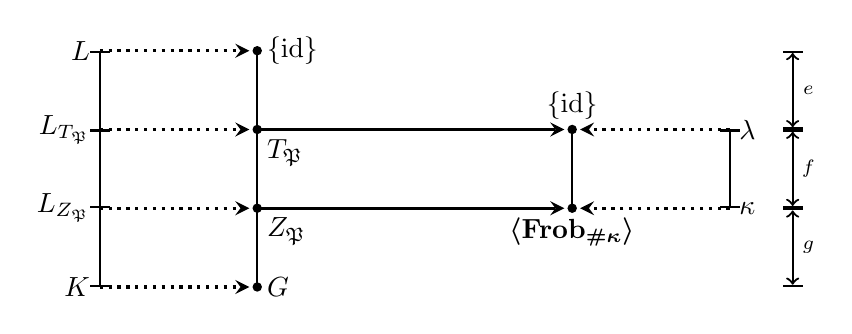
\begin{tikzpicture}
        \coordinate[label=left:$L$] (L) at (-1,1.5);
        \coordinate[label=left:$L_{T_{\mathfrak{P}}}$] (M) at (-1,0.5);
        \coordinate[label=left:$L_{Z_{\mathfrak{P}}}$] (N) at (-1,-0.5);
        \coordinate[label=left:$K$] (K) at (-1,-1.5);
        \coordinate[label=right:$\{\textrm{id}\}$] (id) at (1,1.5);
        \coordinate[label=below right:$T_{\mathfrak{P}}$] (T) at (1,0.5);
        \coordinate[label=below right:$Z_{\mathfrak{P}}$] (Z) at (1,-0.5);
        \coordinate[label=right:$G$] (G) at (1,-1.5);
        \draw[thick] (id)--(G);
        \draw[|-|,thick] (L)--(K);
        \draw[|-|,thick] (M)--(N);
        \draw[->,dotted,very thick,>=stealth] (L)--(0.9,1.5);
        \draw[->,dotted,very thick,>=stealth] (M)--(0.9,0.5);
        \draw[->,dotted,very thick,>=stealth] (N)--(0.9,-0.5);
        \draw[->,dotted,very thick,>=stealth] (K)--(0.9,-1.5);
        \draw[->,very thick,>=stealth] (T)--(4.9,0.5);
        \draw[->,very thick,>=stealth] (Z)--(4.9,-0.5);
        \coordinate[label=above:$\{\mathrm{id}\}$] (id_a) at (5,0.5);
        \coordinate[label=below:$\boldsymbol{\langle\mathrm{Frob}_{\#\kappa}\rangle}$] (frob) at (5,-0.5);
        \draw[thick] (id_a)--(frob);
        \coordinate[label=right:$\lambda$] (lambda) at (7,0.5);
        \coordinate[label=right:$\kappa$] (kappa) at (7,-0.5);
        \draw[|-|,thick] (lambda)--(kappa);
        \draw[->,dotted,very thick,>=stealth] (lambda)--(5.1,0.5);
        \draw[->,dotted,very thick,>=stealth] (kappa)--(5.1,-0.5);
        \fill (id) circle [radius=0.06];
        \fill (T) circle [radius=0.06];
        \fill (Z) circle [radius=0.06];
        \fill (G) circle [radius=0.06];
        \fill (id_a) circle [radius=0.06];
        \fill (frob) circle [radius=0.06];
        \node at (8,1) {\scriptsize$e$};
        \node at (8,0) {\scriptsize$f$};
        \node at (8,-1) {\scriptsize$g$};
        \draw[|<->|,thick] (7.8,0.5)--(7.8,1.5);
        \draw[|<->|,thick] (7.8,-0.5)--(7.8,0.5);
        \draw[|<->|,thick] (7.8,-1.5)--(7.8,-0.5);
    \end{tikzpicture}
    \caption{ヒルベルト理論の対応関係}\label{fig:tikz_field}
\end{figure}

次に,「惰性群」というものを定義する。以降,$\lambda\coloneq\mathcal{O}_L/{\mathfrak{P}},\,\kappa\coloneq\mathcal{O}_K/{\mathfrak{p}}$とする。$x+\mathfrak{P}\in\lambda$と$\sigma\in Z_{\mathfrak{P}}$に対して,$\sigma(x+\mathfrak{P})=\sigma(x)+\mathfrak{P}$となることから,$\sigma$は$\lambda$の自己同型となり,$\sigma$は$\mathcal{O}_K$の元を固定するため$\kappa$の元も固定する。したがって,$\sigma$は$\mathrm{Gal}(\lambda/{\kappa})$の元$\bar{\sigma}$を定め,対応\[
\pi:Z_{\mathfrak{P}}\ni\sigma\mapsto\bar{\sigma}\in\mathrm{Gal}(\lambda/\kappa)
\]が誘導される。$\pi$は単射でない全射準同型となる。そこで,単射にして同型をつくるために,次の群を定義する:
\begin{dfn}[惰性群,惰性体]
    \[
    T_{\mathfrak{P}}\coloneqq\{\sigma\in Z_{\mathfrak{P}}\mid\forall x\in\mathcal{O}_L,\,\sigma(x+\mathfrak{P})=x+\mathfrak{P}\}
    \]とし,$T_{\mathfrak{P}}$を$L/K$における$\mathfrak{P}$の\textbf{惰性群}という.また,$T_{\mathfrak{P}}$の不変体$L_{T_{\mathfrak{P}}}$(ガロアの基本定理により$T_{\mathfrak{P}}$と対応する中間体)を\textbf{惰性体}という.
\end{dfn}
定義から$T_{\mathfrak{P}}=\mathrm{Ker}(\pi)$であるから,群の第一同型定理より,$T_{\mathfrak{P}}$のおかげで$Z_{\mathfrak{P}}/{T_{\mathfrak{P}}}\cong\mathrm{Gal}(\lambda/\kappa)$という同型が得られる。ここで,有限体のガロア理論を思い出すと,$\mathrm{Gal}(\lambda/\kappa)=\langle\mathrm{Frob}_{\#\kappa}\rangle$がわかる(フロベニウス!)。また,$Z_{\mathfrak{P}}$,$Z_{\mathfrak{P}}/{T_{\mathfrak{P}}}$の位数はそれぞれ$ef$,$f$だから,$\# T_{\mathfrak{P}}=e$である。以上で,図\ref{fig:tikz_field}の対応関係が明らかになった。

続いて,体の拡大に対応してどのように素イデアル$\mathfrak{p}$が分解されていくかを見る(おまけ)。$D_{\mathfrak{P}}\coloneqq L_{Z_{\mathfrak{P}}},\; I_{\mathfrak{P}}\coloneqq L_{T_{\mathfrak{P}}}$とする。

まず,$\mathfrak{P}_D\coloneqq\mathfrak{P}\cap\mathcal{O}_{D_{\mathfrak{P}}}$とおくと,$\mathfrak{P}_D\mid\mathfrak{P}$となる。さらに,$\mathfrak{P}_D$の$D_{\mathfrak{P}}/K$における分岐指数,惰性次数を$e',\; f'$とする。同型\eqref{dokei_galois_artin}より,$\mathrm{Gal}(L/D_{\mathfrak{P}})\cong Z_{\mathfrak{P}}$だが,$G$に$\mathrm{Gal}(L/D_{\mathfrak{P}})\cong Z_{\mathfrak{P}}$を当てはめて全単射\eqref{zentan_zp}を考えると,全単射$Z_{\mathfrak{P}}/Z_\mathfrak{P}\rightarrow\{\mathfrak{P}_{D,1},\ldots,\mathfrak{P}_{D,g'}\}$\; ($\{\mathfrak{P}_{D,1},\ldots,\mathfrak{P}_{D,g'}\}$は$\mathfrak{P'}\mid\mathfrak{P}_D$をみたす$\mathcal{O}_L$の素イデアル$\mathfrak{P'}$全体)が得られ,$g'=1$となる。$\mathfrak{P}_D$の$L/{D_{\mathfrak{P}}}$における分岐指数,惰性次数,分解指数はそれぞれ$e/e',\; f/f',\; g'=1$となるから,等式\eqref{toshiki_sp_galois}より,$[L:D_{\mathfrak{P}}]=\frac{e}{e'}\times\frac{f}{f'}\times 1$である。同時に,$[L:D_{\mathfrak{P}}]=\#\mathrm{Gal}(L/D_{\mathfrak{P}})=\# Z_{\mathfrak{P}}=ef$であるから,$e'=f'=1$である。したがって,すべての$\mathfrak{P}_D\mid\mathfrak{p}$の$D_{\mathfrak{P}}/K$における分岐指数と惰性次数が1となり,$\mathfrak{p}$は$D_{\mathfrak{P}}/K$で完全分解する。

次に,$\mathfrak{P}_I\coloneqq\mathfrak{P}\cap\mathcal{O}_{I_{\mathfrak{P}}}$とおく。すると,詳細は省略するが,$\mathcal{O}_{I_{\mathfrak{P}}}/\mathfrak{P}_I=\mathcal{O}_L/\mathfrak{P}$が示せる。したがって,$\mathfrak{P}_I$の$I_{\mathfrak{P}}/D_{\mathfrak{P}}$における惰性次数が$f$であり,等式\eqref{toshiki_sp_galois}と$[I_{\mathfrak{P}}:D_{\mathfrak{P}}]=\# (Z_{\mathfrak{P}}/T_{\mathfrak{P}})=f$より分岐指数が1であることがわかるので,$\mathfrak{P}_D$は$I_{\mathfrak{P}}/D_{\mathfrak{P}}$で惰性する。さらに,等式\eqref{toshiki_sp_galois}から,$\mathfrak{P}_I$が$L/I_\mathfrak{P}$で完全分岐することもわかり,図\ref{fig:tikz_bunkai_p}のようになる。ガロア拡大における素イデアルの分解が具にわかってしまった。
\begin{figure}[ht]
    \centering
    \begin{tikzpicture}
        \coordinate[label=left:$L$] (L) at (-1,1.5);
        \coordinate[label=left:$I_{\mathfrak{P}}$] (M) at (-1,0.5);
        \coordinate[label=left:$D_{\mathfrak{P}}$] (N) at (-1,-0.5);
        \coordinate[label=left:$K$] (K) at (-1,-1.5);
        \draw[|-|,thick] (L)--(K);
        \draw[|-|,thick] (M)--(N);
        \node at (1.2,1) {\scriptsize$e$};
        \node at (1.2,0) {\scriptsize$f$};
        \node at (1.2,-1) {\scriptsize$g$};
        \draw[|->|,>=stealth,thick] (1,0.5)--(1,1.5);
        \draw[|->|,>=stealth,thick] (1,-0.5)--(1,0.5);
        \draw[|->|,>=stealth,thick] (1,-1.5)--(1,-0.5);
        \node[below] at (1,-1.5) {$\mathfrak{p}$};
        \node[right] at (1.2,-0.5) {$\mathfrak{p}\mathcal{O}_{D_{\mathfrak{P}}}=\mathfrak{P}_1'\cdots\mathfrak{P}_g'\, (\mathfrak{P}_1'=\mathfrak{P}_D)$,$\mathfrak{p}$は完全分解};
        \node[right] at (1.2,0.5) {$\mathfrak{P}_D\mathcal{O}_{I_{\mathfrak{P}}}=\mathfrak{P}_I$,$\mathfrak{P}_D$は惰性};
        \node[right] at (1.2,1.5) {$\mathfrak{P}_I\mathcal{O}_L=\mathfrak{P}^e$,$\mathfrak{P}_I$は完全分岐};
        \draw[dotted,thick] (L)--(1,1.5);
        \draw[dotted,thick] (M)--(1,0.5);
        \draw[dotted,thick] (N)--(1,-0.5);
        \draw[dotted,thick] (K)--(1,-1.5);
    \end{tikzpicture}
    \caption{$\mathfrak{p}$の分解のしかた}\label{fig:tikz_bunkai_p}
\end{figure}

\subsection{フロベニウスとともに頂へ}
\textbf{類体論縦走------。}

\vspace{10pt}

この節では,類体論においてフロベニウスがどのように活躍しているかを見る。以下,$\mathfrak{p}$は不分岐とする。

先ほどのヒルベルト理論の帰結として,$Z_{\mathfrak{P}}\cong\mathrm{Gal}(\lambda/\kappa)=\langle\mathrm{Frab}_{\#\kappa}\rangle$が得られた。分解のしかたに関わる分解群を,フロベニウスを通して調べられる,ということだ。
\begin{dfn}[フロベニウス元]
    同型$Z_{\mathfrak{P}}\cong\langle\mathrm{Frab}_{\#\kappa}\rangle$によって$\mathrm{Frob_{\#\kappa}}$と対応する$Z_{\mathfrak{P}}$の生成元を$\left[\frac{L/K}{\mathfrak{P}}\right]$とかき,$L/K$における$Z_{\mathfrak{P}}$の\textbf{フロベニウス元}という.
\end{dfn}
\begin{dfn}[アーベル拡大]
    ガロア拡大$L/K$について,$\mathrm{Gal}(L/K)$がアーベル群(可換群)である時,$L/K$は\textbf{アーベル拡大}であるという.
\end{dfn}
実は,$L/K$がアーベル拡大である時,$Z_{\mathfrak{P}},\; T_{\mathfrak{P}},\; \left[\frac{L/K}{\mathfrak{P}}\right]$は,$\mathfrak{P}\mid\mathfrak{p}$に依らず定まる。そこで,それぞれ$Z_{\mathfrak{p}},\; T_{\mathfrak{p}},\; \left(\frac{L/K}{\mathfrak{p}}\right)$と表す。

フロベニウス元を導入したところで,円分体における素数の分解を考えよう。1の原始$n$乗根を1つ取って$\zeta$とし,円分拡大$\mathbb{Q}(\zeta)/\mathbb{Q}$を考えると,これはアーベル拡大になることが知られている。また,$n=2m\left(2\nmid m\right)$と表せる時,$\mathbb{Q}(\zeta_n)=\mathbb{Q}(\zeta_m)$だから,$n$は奇数または4の倍数であるとして良い。この時,次の事実がある(証明省略):
\begin{prop}
    素数$p$が$\mathbb{Q}(\zeta)/\mathbb{Q}$で分岐することは,$p\mid n$と同値である.
\end{prop}

不分岐の場合を考えていたから,素数$p$と$n$は互いに素とすれば十分である。
\begin{prop}
    $n$と互いに素な素数$p$に関するフロベニウス元$\left(\frac{L/K}{p\mathbb{Z}}\right)$は,$\sigma_p(\zeta)=\zeta^p$という写像$\sigma_p\in\mathrm{Gal}(\mathbb{Q}(\zeta)/\mathbb{Q})$によって定まる.
\end{prop}
\begin{prf}
    $\mathcal{O}_{\mathbb{Q}(\zeta)}=\mathbb{Z}[\zeta]$とフェルマーの小定理,そして$\mathsf{FD}$より,任意の$x=\sum a_i\zeta^i\in\mathbb{Z}[\zeta]$に対し,$\sigma_p(x)+p\mathbb{Z}[\zeta]=\sum a_i(\zeta^p)^i+p\mathbb{Z}[\zeta]=\sum a_i^p\zeta^{pi}+p\mathbb{Z}[\zeta]=(\sum a_i\zeta^i)^p+p\mathbb{Z}[\zeta]=x^p+p\mathbb{Z}[\zeta]$となる.これを満たす写像は一意に定まり,$\sigma_p$はフロベニウス元を定める.
\end{prf}
$\sigma_p$の$\mathrm{Gal}(\mathbb{Q}(\zeta)/\mathbb{Q})$における位数が$f=\# Z_{p\mathbb{Z}}=\#\left\langle\left(\frac{L/K}{p\mathbb{Z}}\right)\right\rangle$を与えるから,$\sigma_p$の位数を求めたい。ここで,同型による対応$\mathrm{Gal}(\mathbb{Q}(\zeta)/\mathbb{Q})\ni\sigma_p\mapsto\bar{p}\in (\mathbb{Z}/n\mathbb{Z})^{\times}$があったから,$\sigma_p$の位数$f$は,$\bar{p}$の$(\mathbb{Z}/n\mathbb{Z})^{\times}$における位数に等しいことがわかり,次のようになる:
\begin{thm}
    $n$と互いに素な素数$p$に対し,$p^f\equiv 1\pmod{n}$を満たす最小の正整数$f$により,$p$は\[
    p\mathbb{Z}[\zeta]=\mathfrak{p}_1\mathfrak{p}_2\cdots\mathfrak{p}_{[\mathbb{Q}(\zeta):\mathbb{Q}]/f}=\mathfrak{p}_1\mathfrak{p}_2\cdots\mathfrak{p}_{\varphi(n)/f}
    \]と分解する.
\end{thm}
こうして,円分体での素数の分解法則が記述できた。平方根を添加した体における素数の分解法則を直接考えた際に比べて,議論が簡潔である。フロベニウスのおかげである。元を辿れば,フロベニウス写像が準同型であることの背景に\textsf{FD}があった。類体論を前にして\textsf{FD}の存在は些末かもしれないが,\textsf{FD}がなければここまで来れなかった。中高生の習う数学で間違いとされていることを肯定することで生まれる可能性がある,ということを示したかった。

円分体やフロベニウスに関連して,類体論そのものについて少し述べておこう。

ガロア拡大$L/K$を考える。$\mathcal{O}_K$の素イデアル$\mathfrak{p}$が$L/K$で不分岐する時,フロベニウス元が$\mathrm{Gal}(L/K)$の元として定まることを考えると,いろいろな$\mathfrak{p}$に対してフロベニウス元が対応することで,$\mathrm{Gal}(L/K)$や$L/K$そのものの構造がわかってしまうのではないか,と考えられる。実際に,任意の$\mathrm{Gal}(L/K)$の元は,$\mathcal{O}_K$のある不分岐する素イデアル$\mathfrak{p}$に対応するフロベニウス元として表されるのだ。これを使うと,$L/K$がアーベル拡大の時,\[
\bigoplus_{\mathfrak{p}}\mathbb{Z}\ni (n_{\mathfrak{p}})_{\mathfrak{p}}\mapsto\prod_{\mathfrak{p}}\mathrm{Frob}_{\mathfrak{p}}^{n_{\mathfrak{p}}}\in\mathrm{Gal}(L/K)
\]という群準同型($\oplus$は(外部)直和というもの,調べてね)が全射となり,第一同型定理より,この写像の核を理解することで$\mathrm{Gal}(L/K)$の構造がわかってしまうという(まだそこまで勉強できてないから結果だけ)。また,このような写像はアルティン写像というもので,アルティンの相互法則というアルティン写像の核に関する法則があり,``$n$乗剰余の相互法則''を導くのに使ったり,類体論において大事なことが沢山わかったりするらしい。

さらに,円分体については次の素晴らしい定理がある:
\begin{thm}[クロネッカー-ウェーバーの定理]
    $\mathbb{Q}$の任意のアーベル拡大は,ある円分体$\mathbb{Q}(\zeta)$の部分体となる.
\end{thm}
代数体の拡大を考える上で,円分体は大事な対象だったのだ。

ところで,「類体論」ってなんだろう。代数的整数論に属する分野で,凡そ今まで述べてきたアーベル拡大に関する議論などを精緻化した,理論体系のことを言うのだろう(「非可換類体論」というのもあるようだ)。しかし,私はまだ勉強し始めたばかりなので,まだ「類体論とは何か」に答えを出さないでおく。類体論についての内容おわり$\diamond$










\section{リュカの定理とシェルピンスキーのギャスケット}

ここでは,\textsf{FD}から導かれるリュカの定理によって,パスカルの三角形を色分けしたものである「シェルピンスキーのギャスケット」を効率的に表示するアルゴリズムを作成する。また,Pythonを用いる。

\subsection{リュカの定理}
\begin{thm}[Lucas]
    非負整数$n,m$と素数$p$に対し,$0 \leqq n_i< p$の下で,\[
    n=n_kp^k+n_{k-1}p^{k-1}+\cdots+n_0p^0,\,m=m_kp^k+m_{k-1}p^{k-1}+\cdots+m_0p^0
    \]
    とする.このとき,\[
    \binom{n}{m}\equiv \prod_{i=0}^{k} \binom{n_i}{m_i} \quad \mathrm{mod}\, p
    \]
    である.ただし,$a<b$に対しては$\binom{a}{b}=0$とする.
\end{thm}

これがリュカの定理である。実はこれは,補題\ref{mod_fresh}を用いて示すことができる。具体的には,次の補題を用いる。
\begin{lemma}[\textsf{FD}]\label{mod_fresh_sec}
    $x\in\mathbb{Z}$に対し,$(1+x)^{p^i}\equiv 1+x^{p^i} \quad \mathrm{mod}\,p$である.
\end{lemma}

この補題は補題\ref{mod_fresh}を繰り返し用いれば容易に示せる。

それでは,この補題を使ってリュカの定理を証明していこう:
\begin{prf}
    $(1+x)^n$を展開した時の$x^m$の係数に注目することで示す.

    まず,$(1+x)^n=\prod_{i=0}^{k}(1+x)^{n_ip^i}\equiv\prod_{i=0}^{k}(1+x^{p^i})^{n_i}\quad \mathrm{mod}\,p$となる.また,$m=m_kp^k+m_{k-1}p^{k-1}+\cdots+m_0p^0$という表示の一意性より,最右辺で$x^m$という項が登場するのは,$(1+x^{p^k})^{n_k}$から$x^{m_kp^k}$,$(1+x^{p^{k-1}})^{n_{k-1}}$から$x^{m_{k-1}p^{k-1}}$,\dots,$(1+x^{p^0})^{n_0}$から$x^{n_0}$,を選出したもののみなので,$x^m$の係数は,$\prod_{i=0}^{k}\binom{n_i}{m_i}$である.よって,法$p$の下,$\binom{n}{m}\equiv\prod_{i=0}^{k}\binom{n_i}{m_i}$である.
\end{prf}

少々技巧的な証明だが,\textsf{FD}の威力が存分に発揮されているのが見て取れる。

ここで少し定理の条件に触れておく。$n=n_kp^k+n_{k-1}p^{k-1}+\cdots+n_0p^0,\,m=m_kp^k+m_{k-1}p^{k-1}+\cdots+m_0p^0$という表示は$p$進法を想起させる。コンピュータは2進法で動いてるよ,とかの話で出てくるアレだ。実際にその通りで,条件は$p$を基数としたときに$n=n_kn_{k-1}\cdots n_0,m=m_km_{k-1}\cdots m_0$であることと同じである。

\subsection{シェルピンスキーのギャスケット}
まず,シェルピンスキーのギャスケットについて説明する。

一言で言うと,パスカルの三角形を色分けしたものだ。一般的には偶奇で色分けしたものを言う。しかし,そもそもシェルピンスキーのギャスケットは,どれだけ拡大しても同じ構造が現れてくる「フラクタル図形」の一種である点が重要である。一度ネットなどで画像を調べたり,自分でパスカルの三角形を塗り分けてみたりして,その容貌を目に焼き付けてからこれ以降の内容を読んで欲しい(図\ref{sierp_2_and}を見てもらっても構わない)。

\vspace{10pt}

シェルピンスキーのギャスケットを表示する際に問題となるのは,二項係数の偶奇を判定する方法である。素朴にやるのであれば,\texttt{\textbf{import} math}のもとで\texttt{math.comb(n,m) \% 2}をひたすら計算すれば良いが,これでは,ギャスケットの段数が大きくなった時に時間がかかってしまう。そこで,リュカの定理をうまく使う。そのまま使うと,一度2進法に直したものを2で割ったあまりを求めて掛け合わせなければならないが,プログラム\ref{sierpinski}に示したアルゴリズムはより速いものである。なお,これに関係するプログラムと一緒に別のGitHubリポジトリ(\url{https://github.com/stochastic-yukke/python-sierpinski-gasket})の中にも置いておきました。

\begin{lstlisting}[caption=uszczelka Sierpińskiego,label=sierpinski]
import matplotlib.pyplot as plt
import numpy as np

def binomial_odd(n: int, k: int):
    return (n & k) == k

def lucas_mod2_triangle(rows):
    triangle = np.zeros((rows, 2 * rows - 1), dtype=int)
    for n in range(rows):
        for k in range(n + 1):
            col = rows - n + 2 * k - 1
            triangle[n, col] = binomial_odd(n, k)
    return triangle

def plot_sierpinski_lucas(rows):
    data = lucas_mod2_triangle(rows)
    fig, ax = plt.subplots(figsize=(8, 8))
    ax.imshow(data, cmap='binary', interpolation='nearest')
    ax.axis('off')
    return fig

# 図を生成して表示
fig = plot_sierpinski_lucas(256)
plt.show()
\end{lstlisting}

結果は図\ref{sierp_2_and}のようになる。
\begin{figure}[ht]
    \centering
        \includegraphics[scale=0.5]{../figures/Figure_using_and.png}
    \caption{シェルピンスキのギャスケット(mod2, rows=256)}
    \label{sierp_2_and}
\end{figure}

このプログラムにおいて注目して欲しいのは,4-5行目の関数\texttt{binomial\_odd}である。\texttt{\&}というのは,「論理積」を意味する。自然数$n$と$k$を二進法表記したときの$i+1$桁目の数の組$(n_i,k_i)$が$(1,1)$のときのみ1を,そうでないとき0を,その$i$桁目とするような数を,再び10進法にしたものが$n,k$の論理積である。例えば,$7=0111{}_{(2)},\,11=1011{}_{(2)}$だから,各桁を比較することで\texttt{7\&11}は$0011{}_{(2)}=3$であるとわかる。

$n,m$を$k+1$桁に二進展開したときの$i+1$桁目$n_i,m_i$に対する$\binom{n_i}{m_i}$としてありうるのは$\binom{1}{1}=1,\binom{1}{0}=1,\binom{0}{1}=0,\binom{0}{0}=1$のみであるから,リュカの定理より,$(n_l,m_l)=(0,1)$となるような整数$0\leqq l \leqq k$が存在する時,かつそのときに限り,$\binom{n}{m}\equiv 0 \quad \mathrm{mod}\,2$となる。したがって,$(n_l,m_l)=(0,1)$となる$l$の有無によって二項係数の偶奇を判定すればよい。実はここで,$\mathtt{\&}$が活躍する。$(n_l,m_l)$に対し,$n_l,m_l$の論理積を計算することを考えると,$n_l\mathtt{\&}m_l\ne m_l$となるのは,$(n_l,m_l)=(0,1)$のとき,かつその時に限るから,$n\mathtt{\&}m$の桁で,$m$の対応する桁と一致しないものが1つでもあれば,$\binom{n}{m}\equiv 0\quad \mathrm{mod}\,2$となり,$n\mathtt{\&}m$が$m$と一致するならば,$\binom{n}{m}\equiv 1\quad\mathrm{mod}\,2$となる。そういうわけで,このプログラムでは論理積によって二項係数の偶奇を判定しているのである。

\subsection{素数判定アルゴリズム「AKS判定法」の紹介}
\textsf{FD}が効果的に用いられている素数判定法がある。\textbf{AKS判定法}だ。今回は紹介するに留めるが,素数判定の歴史から鑑みても非常に重要なアルゴリズムである(\textbf{史上初の多項式時間で判定可能な決定的素数判定アルゴリズム})。

最も初等的な素数判定のやり方は,フェルマーの小定理を用いる「フェルマーテスト」だが,これでは完全に素数のみを抽出するアルゴリズムとは言えない(フェルマーの小定理の条件を考えればわかる)。このような,素数と合成数をきっぱり峻別できないようなアルゴリズムとは異なり,AKS判定法は確定的に素数を判定できる優れものだ。それでは,アルゴリズムの詳細を以下に示そう:

整数$n>1$に対して,
\begin{enumerate}
    \item $a\in \mathbb{N}が存在してn=a^bかつb>1$ならば「$n$は合成数」と出力して終了.
    \item $\mathrm{ord}_r(n)>\log^2n$をみたす最小の$r$を見つける.
    \item ある$a\leqq r$に対して,$1<(a,n)<n$であるならば「$n$は合成数」と出力して終了.
    \item $n\leqq r$ならば「$n$は素数」と出力して終了.
    \item $a$を$1$から$\lfloor\sqrt{\varphi(r)}\log n\rfloor$まで動かす.$(X+a)^n\not\equiv X^n+a \pmod {X^r-1,n}$ならば「$n$は合成数」と出力して終了.
    \item 「$n$は素数」と出力して終了.
\end{enumerate}

ただし,$(\cdot ,\cdot)$は二数の最大公約数,$\lfloor\cdot\rfloor$は床関数(その数を超えない最大の整数を示す記号),$\varphi$はオイラー関数(正整数$n$に対し,$n$と互いに素な1以上$n$以下の正整数の個数を与える関数)である。また,正整数$x$に対して,$\mathrm{ord}_r(x)$は,法$r$における$x$の位数である(定義\ref{def_genshikon}参照のこと)。

アルゴリズムの5. において\textsf{FD}が輝いているのが見えるだろうか。あれが星というものである。





\section{参考にした文献と参考になるであろう文献}\label{bib}
\cite{yukie}--\cite{tsuji}は,この記事を書く上で(多少なりとも)参考にした資料。一方,\cite{suron}--\cite{frak3}は,記事を書く上でほとんど参照していないが,読者の参考になるかもしれない文献。

\cite{modern_integers}は,初等整数論に始まり,代数的整数論や解析的整数論の基礎的な内容と展望が,テンポよく述べられている本である。理想数のアイデアが詳しく載っていた。
\cite{susemi}は,文章が千夜一夜物語を意識した小説風になっている,楽しい記事である。\cite{intro}は,「類体論の心と七五三の心は通ずるものがあると思ったのです」など印象的な部分が多く,わかりやすく伝えるにはどうすれば良いか考える際に参考になった。
\cite{primes_p}は,AKS判定法についての論文。\cite{suron}は,どこ/いつだったかは忘れたが,一部読んだことがあった本。「岩波講座 現代数学の基礎」シリーズの『数論1』『数論2』をまとめたもの。絶版になっているので,どこかの図書館で借りるか神田の明倫館書店で買うかしよう。
\cite{frak1}は,ドイツの書字をめぐって,歴史や教育について述べている。\cite{frak2}は,印刷博物館の「黒の芸術」展に寄せて学芸員の方が書いたもの。urlにwwwを含めないと開けないようだ。\cite{frak3}には,SütterlinによるKurrent(ドイツの筆記体)やFrakturをはじめとする古典的なドイツの書字が使われなくなったことなどについて,歴史と考察が書かれている。

今回の記事執筆を通して,図書館というインフラの重要性を認識した。

すべて,最終閲覧日は2026年1月3日である。また,「参考になるであろう文献」すなわち\cite{suron}以降の文献は,変更したり追加したりする可能性がある。

\begin{thebibliography}{9}
%%% 今回はbibtexを使わなかった %%%
    \bibitem{yukie} 雪江明彦,『整数論1 初等整数論から$p$進数へ』,日本評論社(2013).
    \bibitem{modern_integers} 落合理,『現代整数論の風景 素数からゼータ関数まで』,日本評論社(2019).
    \bibitem{susemi} 原隆,『数学セミナー』「数の世界の千一夜」第3回,第5回--第7回,日本評論社(2022).
    \bibitem{intro} 加藤和也,『数論への招待』,丸善出版(2012).
    \bibitem{tsudoi} YouTube『すうがく徒のつどい@オンライン「代数的整数論 類体論入門」』,alg-d,\\
    \url{https://www.youtube.com/watch?v=MtFluwn36bk}
    \bibitem{primes_p} Manindra Agrawal, Neeraj Kayal, Nitin Saxena, \emph{PRIMES is in P}, Annals of Mathematics, \textbf{160} (2004), 781--793,\\
    \url{https://annals.math.princeton.edu/wp-content/uploads/annals-v160-n2-p12.pdf}
    \bibitem{frobenius_kurims} 越川皓永,『Frobenius写像の周辺』第42回 京都大学数理解析研究所 数学入門講座(2021),\\
    \url{https://www.kurims.kyoto-u.ac.jp/~kenkyubu/kokai-koza/R3-koshikawa.pdf}
    \bibitem{tsuji} 『素イデアル分解法則を考える(ヒルベルトの理論とフロベニウス自己同型)』,tsujimotterのノートブック,\\
    \url{https://tsujimotter.hatenablog.com/entry/hilbert-theorem}
    \bibitem{suron} 加藤和也, 黒川信重, 斎藤毅,『数論I Fermatの夢と類体論』,岩波書店(2005).
    \bibitem{yellow} 著:J.ノイキルヒ,監訳:足立恒雄,訳:梅垣敦紀,『代数的整数論』,丸善出版(2012).
    \bibitem{yukie2} 雪江明彦,『整数論2 代数的整数論の基礎』,日本評論社(2013).
    \bibitem{alg} alg-d,『代数的整数論 類体論』(2013),\\
    \url{https://alg-d.com/math/number\_theory/class\_field\_theory.pdf}
    \bibitem{frak1} 深井里奈子,『ドイツにおける筆記体の変遷と手書き文字に求められる役割 : 初等学校の書字教育を参考に』,千葉大学大学院人文社会科学研究科研究プロジェクト報告書,\textbf{299} (2016), 86--99,\\
    \url{https://opac.ll.chiba-u.jp/da/curator/100347/BA31027730_299_p086_FUK.pdf}
    \bibitem{frak2} 式洋子,印刷博物館ニュース Vol.96 特集1『特集「黒の芸術」解題』,印刷博物館(2025),\\
    \url{https://www.printing-museum.org/etc/pnews/09601.php}
    \bibitem{frak3} ``A History of the Old German Script'', Walden Font Co.(2019),\\
    \url{https://blog.waldenfont.com/2019/06/26/the-history-of-the-old-german-script/}
\end{thebibliography}

\section{追記}
p.10のフラクトゥーアについて書いた部分の正しさを支える参考文献がないことに気づきました。おそらく,自分の記憶だけをもとに書いてしまったと思われます。書いてあることは概ね正しかったのですが,参考文献を掲載した方が良いと感じたので,追加しました。言葉遣いも断定調でなく「とされている」というふうにしておきました。

フラクトゥーアに関する参考文献は,\cite{frak1}--\cite{frak3}です。

\end{document}
